\section{Induce subdivision}
\label{section:pl-subdivide}

The goal of subdividing $N$ is to create and identify handle attachment sites analogous to the face, edge, and vertex blocks of Chapter \ref{chapter:smooth}.
We use a similar technique to that found in Chapter \ref{chapter:smooth}, iteratively subdividing the tetrahedra of $N$ by certain preimages of $f$.
Tetrahedron subdivisions are compatible, i.e.\ tetrahedron subdivisions fit together exactly as the undivided tetrahedra do inside of $N$.

Let $\sigma$ be a tetrahedron of $N$ and let $s$ be a line segment in the plane such that $s\cap f(\sigma)$ is nonempty, the endpoints of $s$ are outside of $f(\sigma)$,  and $s\cap f(\sigma)$ is a line segment in $f(\sigma)$ disjoint from any vertices or crossings of $f(\sigma)$.
Figure \ref{fig:standard-position-intersection} demonstrates the possible configurations of these line segments, and shows that their preimages inside of $\sigma$ are triangles and quadrilateral (or \emph{quads}).
We refer to these preimages as \emph{exterior triangles} and \emph{exterior quads}.
When a pair of these preimages intersect, the intersection is a line segment with endpoints interior to a pair of triangles of $\sigma^2$.

\begin{figure}[h!]
	\centering
	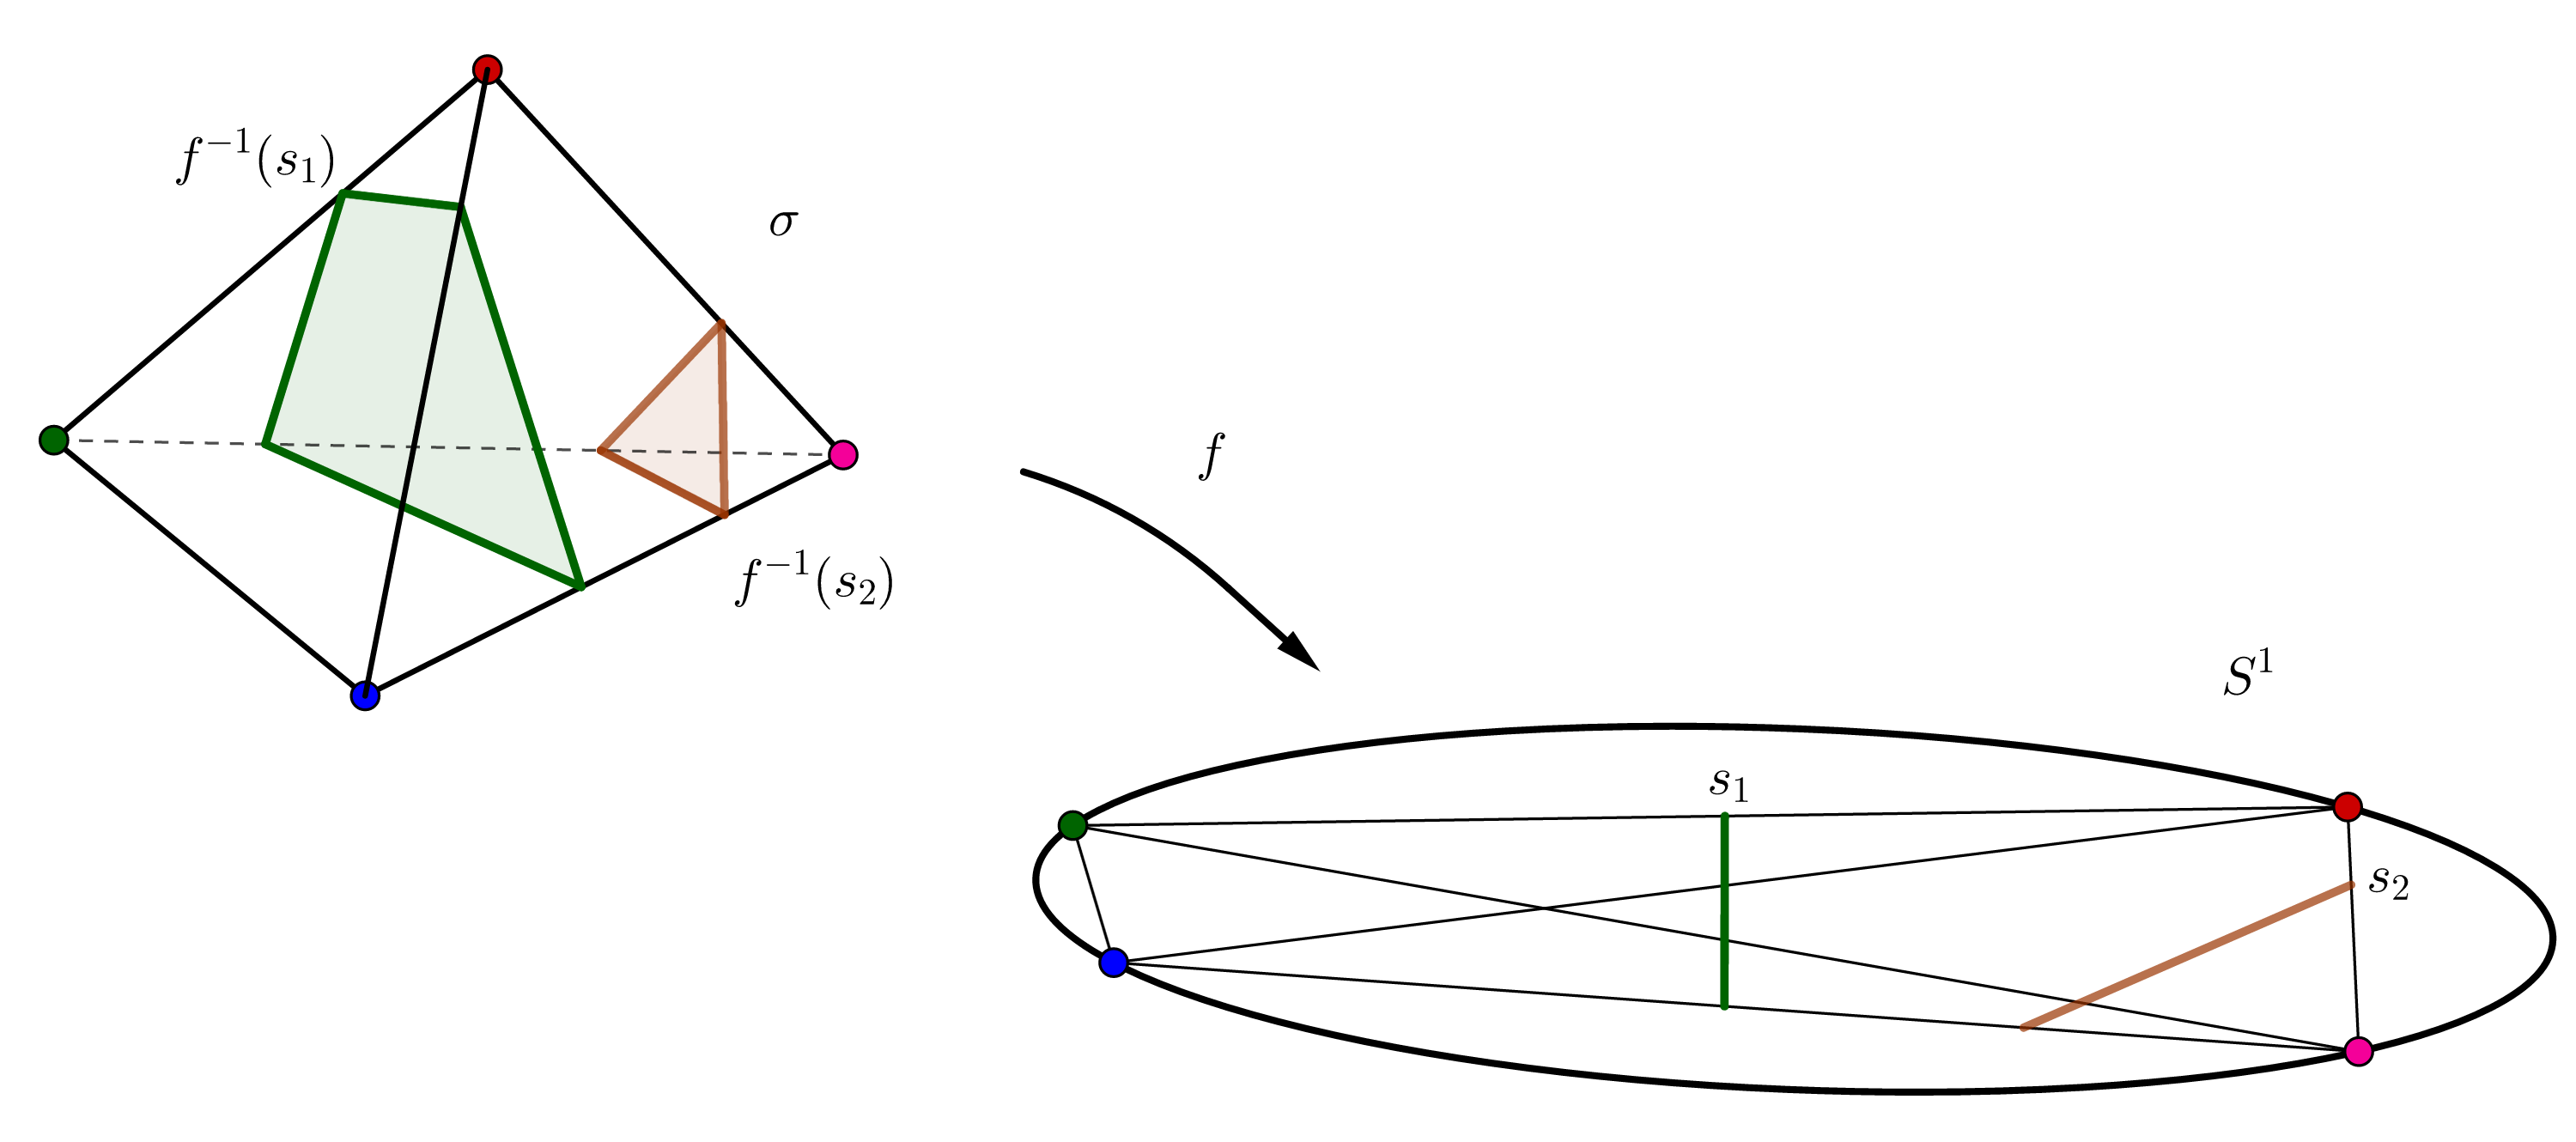
\includegraphics[width=0.9\textwidth]{figures/standard-position-intersection.png}
	\caption{
		\textbf{A tetrahedron $\sigma$ in standard position, intersecting edges, and preimage triangles and quads.}
		An intersecting edge separates the vertices of $\sigma$.
		If one is separated from the other three, its preimage is a triangle.
		If the vertices are separated into two pairs of two, the preimage is a quad.
	}
	\label{fig:standard-position-intersection}
\end{figure}

For each $\sigma\in N^3$ and each edge $e$ of $N^1$ such that $e\notin\sigma^1$, $f(e)$ is a line segment in the plane that is either disjoint from $f(\sigma)$ or induces an exterior triangle or quad in $\sigma$.
%There are two edges of $\sigma$ whose preimages in $\sigma$ form \emph{interior triangles} and these are the \emph{interior edges} of $\sigma$.
The image of $\sigma$ is a quadrilateral in the plane, and four of $\sigma$'s edges map to the boundary of that quadrilateral.
The remaining two edges are the \emph{interior edges} of $\sigma$, and the subdividing preimage triangles they induce in $\sigma$ are \emph{interior triangles}.
%These are the preimages of the edges of $\sigma$ that map through $f$ across $f(\sigma)$ as in Figure \ref{fig:standard-position}, and we refer to these edges as \emph{interior edges}.
%The three edges of the interior triangle induced by $e$ are $e$ itself along with a pair of edges that bisect the triangles of $\sigma$ not containing $e$ as an edge.
%The three vertices of the interior triangle induced by $e$ are the two vertices of $\sigma$ that are the endpoints of $e$ along with a third vertex located in the edge of $\sigma$ opposite $e$.
Figure \ref{fig:standard-position-interior-exterior} shows one interior triangle along with its possible intersections with exterior triangles and quads.
The interior triangles of $\sigma$ always intersect in a line segment with endpoints inside of the interior edges of $\sigma$, shown in Figure \ref{fig:standard-position-interior-interior}

\begin{figure}[h!]
	\centering
	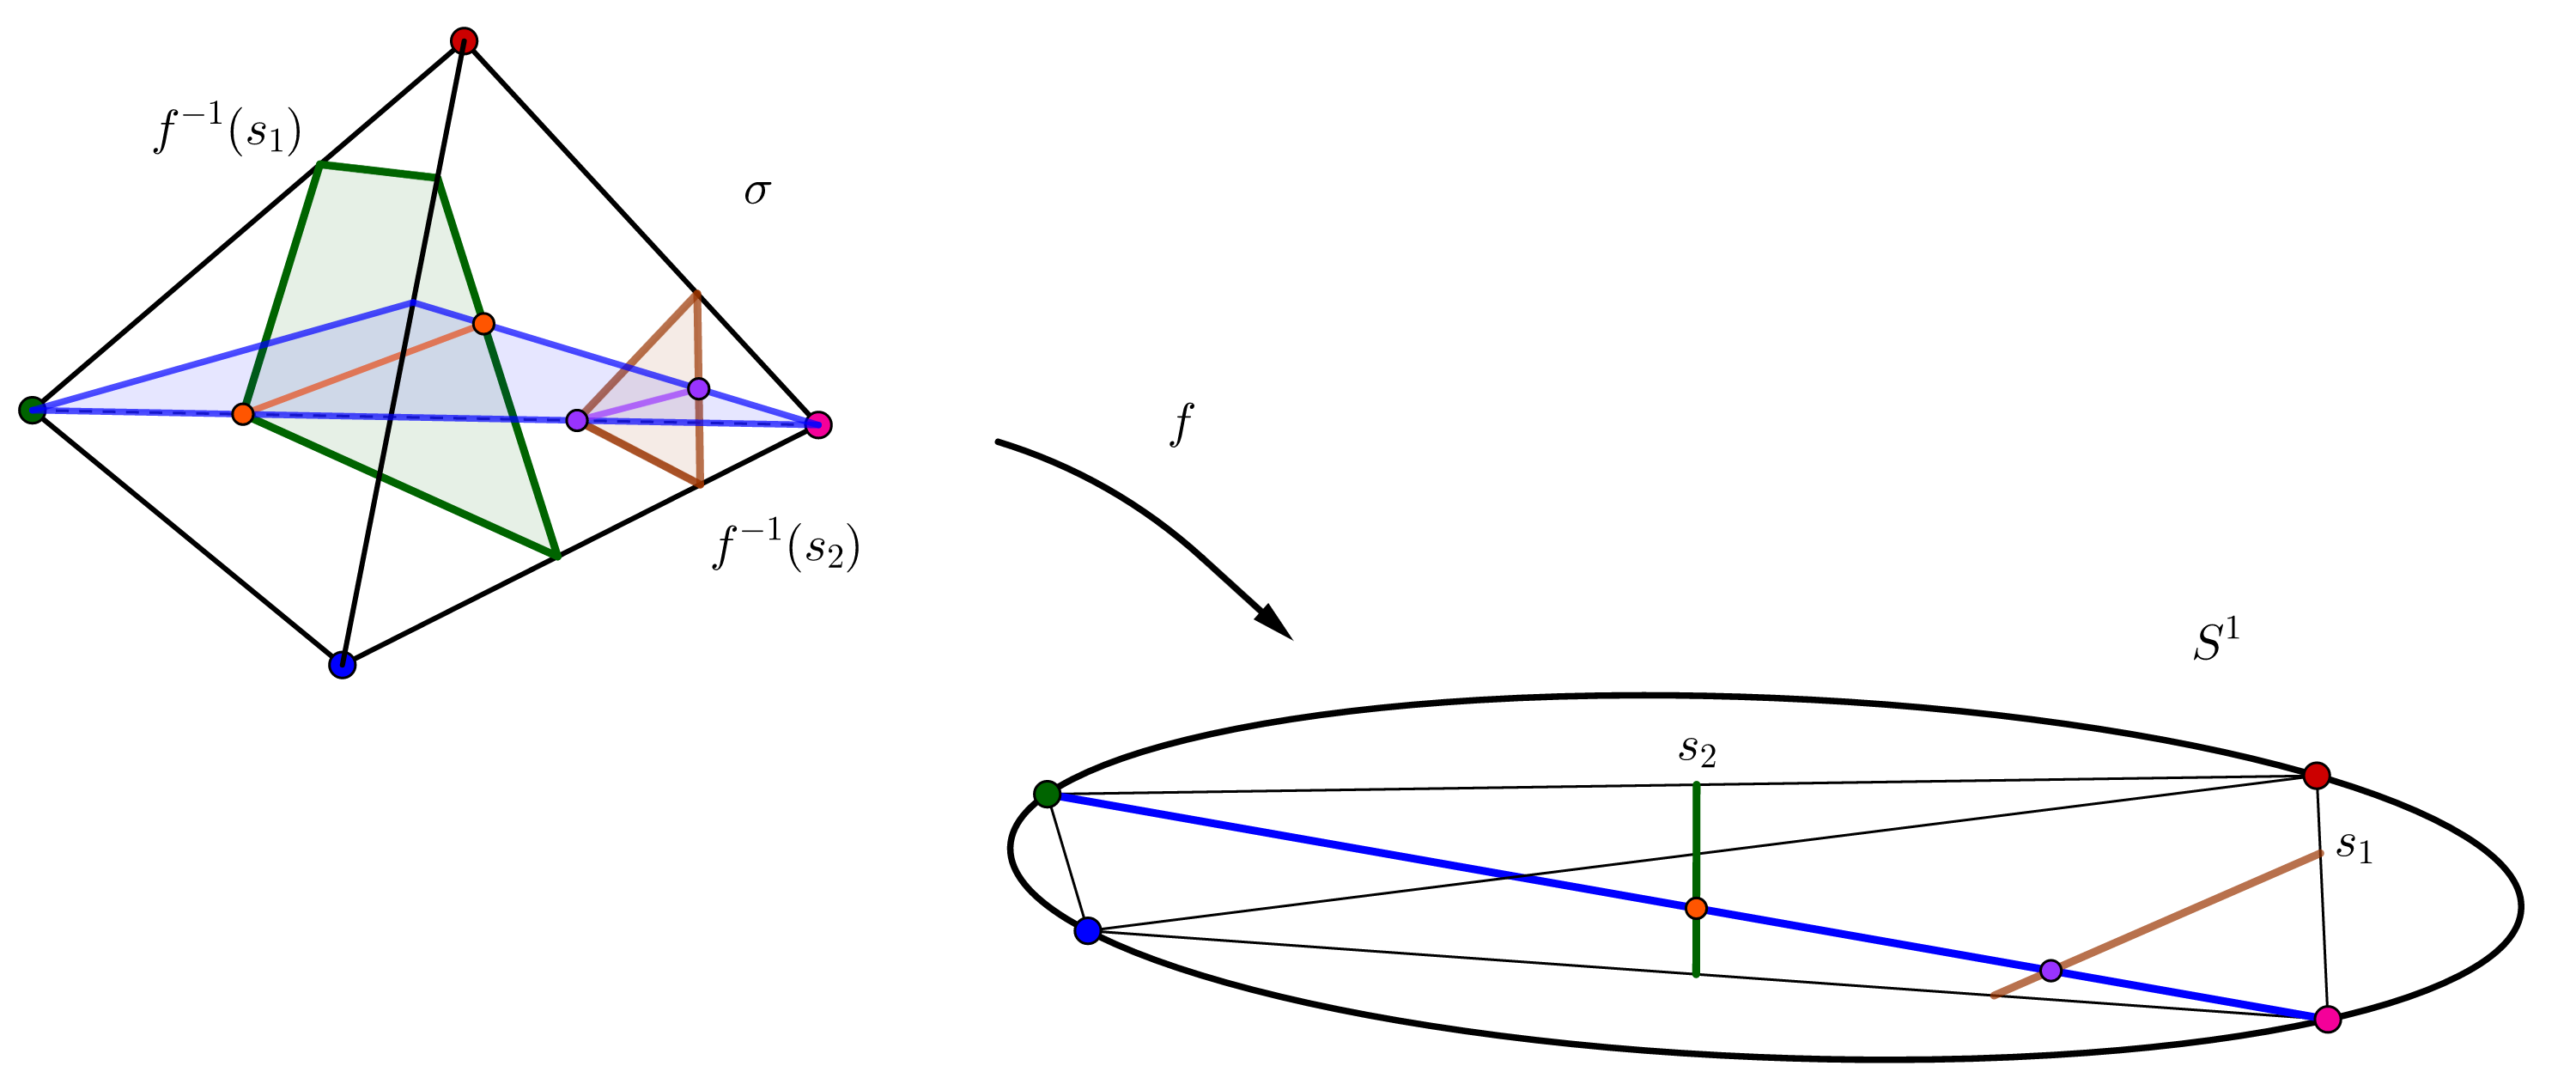
\includegraphics[width=0.9\textwidth]{figures/standard-position-interior-exterior.png}
	\caption{
		\textbf{A tetrahedron $\sigma$ in standard position, one interior triangle, one exterior triangle, and one exterior quad.}
		There are two special preimage triangles in $\sigma$, called \emph{interior triangles}, that occur as the preimages of the edges of $\sigma$ that map through $f$ across $f(\sigma)$ as in Figure \ref{fig:standard-position}.
	}
	\label{fig:standard-position-interior-exterior}
\end{figure}

\begin{figure}[h!]
	\centering
	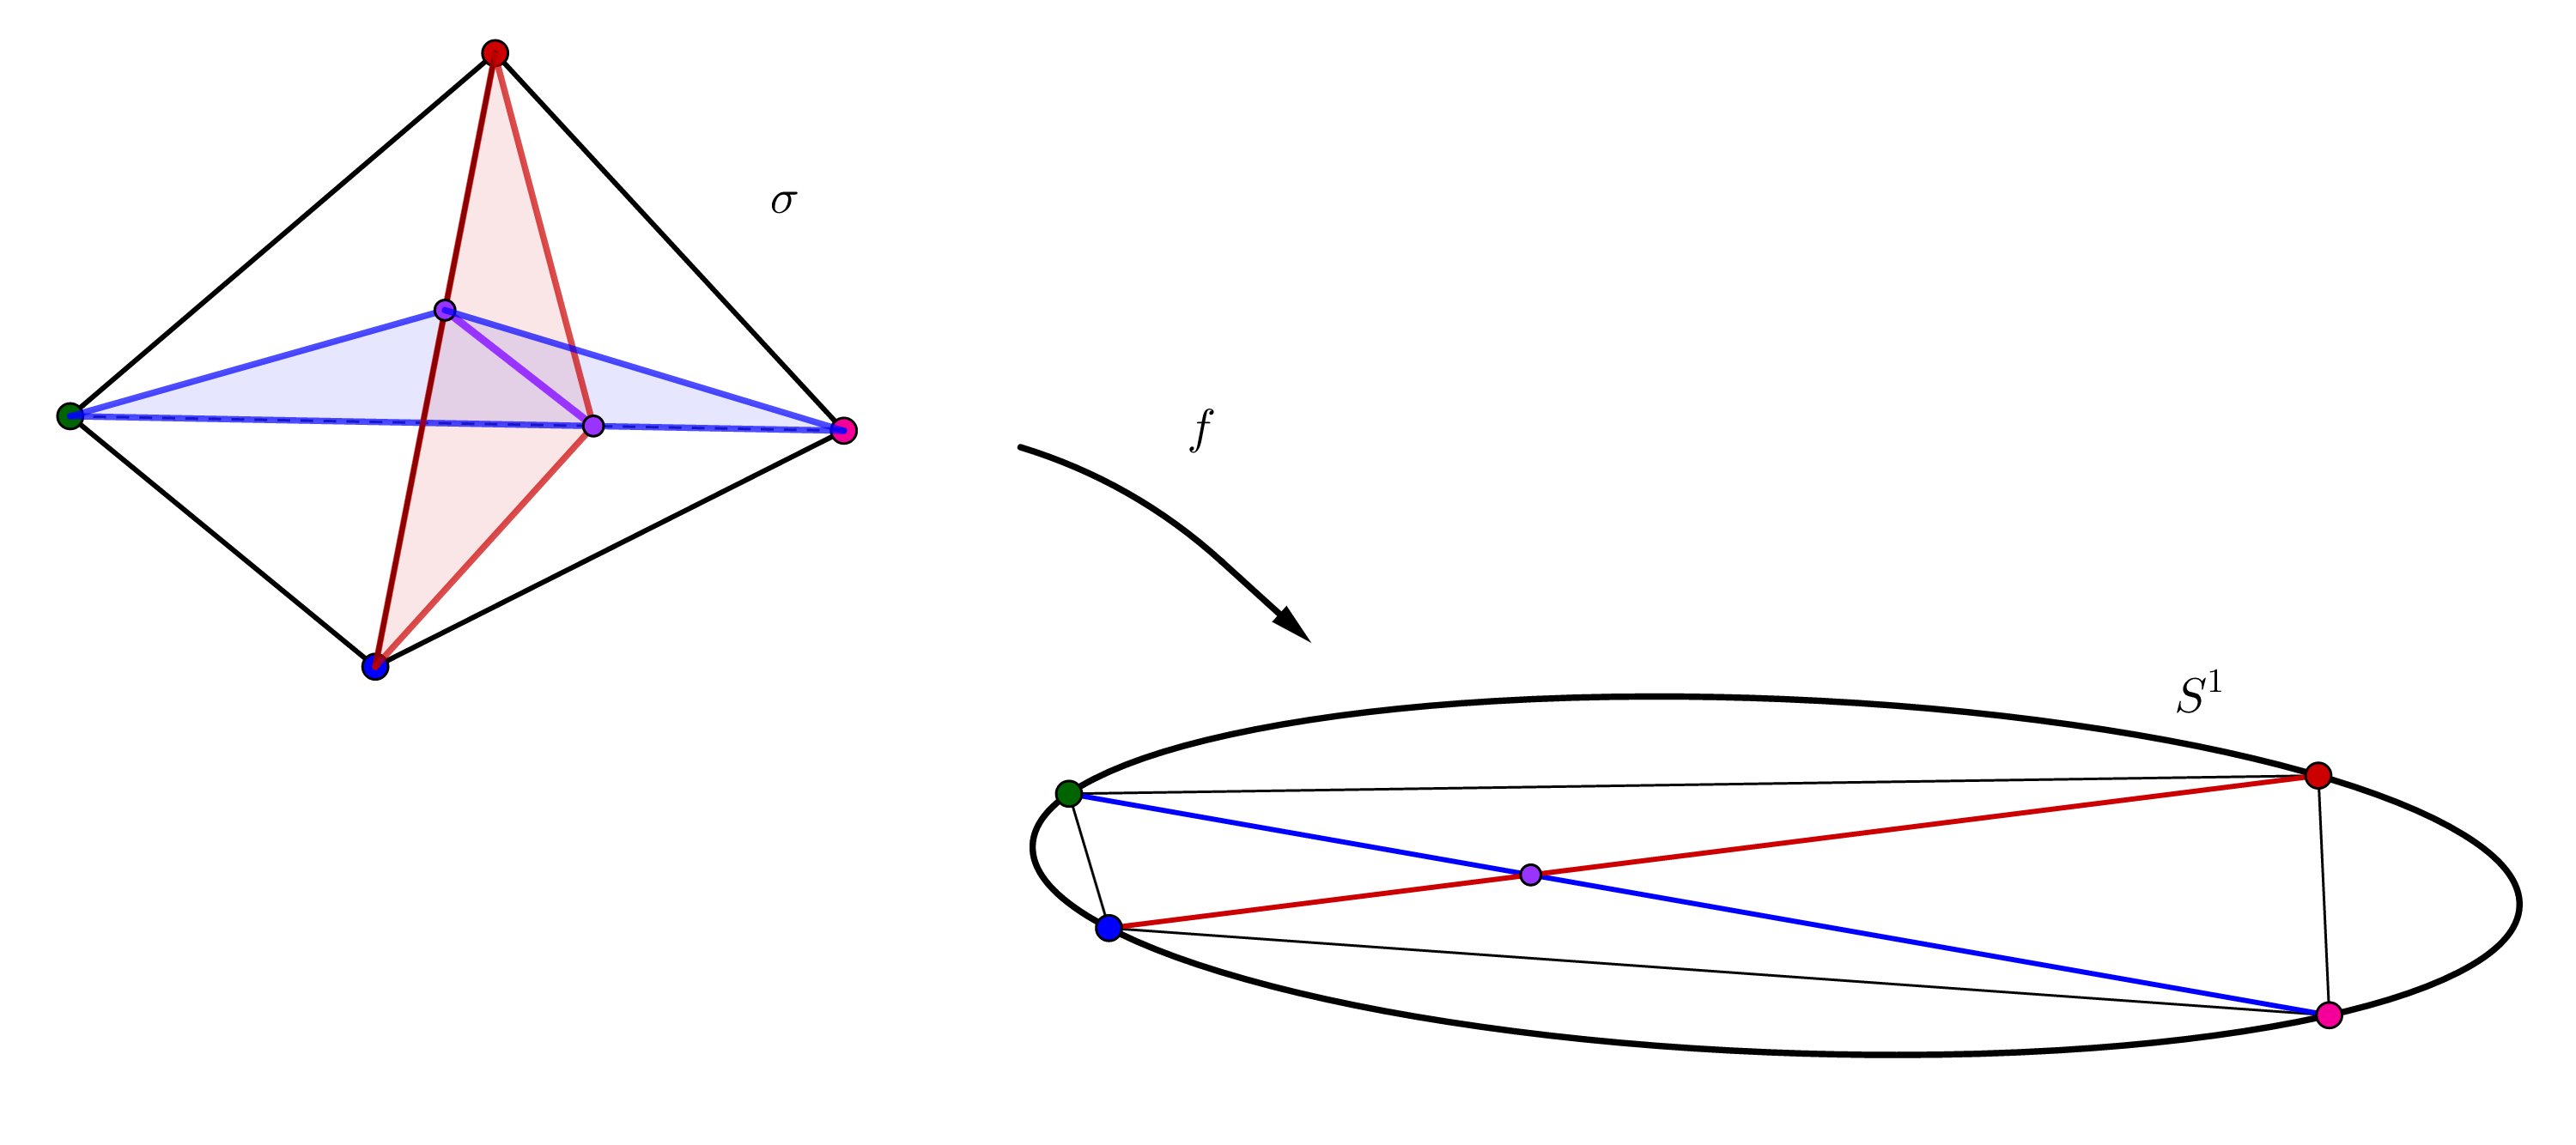
\includegraphics[width=0.9\textwidth]{figures/standard-position-interior-interior.png}
	\caption{
		\textbf{A tetrahedron $\sigma$ in standard position with both interior triangles.}
		As in Figure \ref{fig:standard-position-interior-exterior}, but displaying both interior triangles.
	}
	\label{fig:standard-position-interior-interior}
\end{figure}

Recall that the goal of this subdivision is to identify combinatorial analogues for the face, edge, and vertex blocks of Chapter \ref{chapter:smooth}.
If we were to subdivide $N$ using the quads and triangles induced by the edges of $N$, such blocks are ill-defined.
We amend this by introducing a set of line segments analogous to the sleeves of Section \ref{section:smooth-decompose}.

The vertices of $N$ are sent to the edge of the boundary of the disc in the plane, and this boundary is the only location in the plane where our smooth singularity theory does not apply.
Our first set of line segments remedies this.
Let $p$ be a vertex of $N$ and $s$ a secant in the disc that separates $f(p)$ from $f(N^0\setminus{p})$.
Then $f\inv(s)$ is a triangulated 2--sphere, and is the boundary of a triangulated 3--disc centred at $p$.
We use such 3--discs as our first collection of combinatorial vertex blocks

The vertices of $N$ are mapped to the $k\nth$ roots of unity and the rest of the simplices of $N$ are mapped to the plane via linear extension.
Consider the regular $k$--gon $G_k$ with vertices the $k\nth$ roots of unity reflected through the origin.
Because $k$ is odd, each of $G_k$'s edges is a secant in the disc that separates the image of one vertex of $N$ from the rest.
Moreover, $G_k$ separates $f(N^0)$ from the interior edge-edge crossings of $f(N)$.
We use $G_k$ as our first set of line segments.

Next, we introduce segments that induce the edge and face blocks and the rest of the vertex blocks.
For each edge $e$ of $N^1$, consider $e_\varepsilon^+ = s(e+\varepsilon_e e_\perp)$ and $e_\varepsilon^- =s(e-\varepsilon_e e_\perp)$, secants in $G_k$ that are parallel to $f(e)$ and located a small orthogonal distance away from $f(e)$.
Here we are using $s(\cdot)$ as a function that extends and trims line segments in the plane into secants in $G_k$.
We require that our $\varepsilon$'s are small enough that if $e,g\in N^1$ share a boundary vertex then $e_\varepsilon^\pm$ and $g_\varepsilon^\pm$ do not intersect (i.e. $G_k$ truncates the segments so that their intersection occurs outside of $G_k$).
%the rectangle $R_e$ in the plane defined by $e_\varepsilon^+$ and $e_\varepsilon^-$ does not fully contain $g_\varepsilon^\pm$ for any $g\in N^1$.
%This requirement also ensures that the only crossings of $f(N^1)$ contained in $R_e$ are crossings involving $e$.
The segments $e_\varepsilon^\pm$ for each $e\in N^1$ are called \emph{sleeve segments}, and their preimages form exterior triangles and quads inside of the tetrahedra of $N$.
Figure \ref{fig:pl-segments} depicts the inclusion of $G_k$ and all sleeve segments for a mapping of a triangulated $S^3$ to the plane.
Here, the triangulation of $S^3$ used is the 2-tetrahedron triangulation.

\begin{figure}[h!]
	\centering
	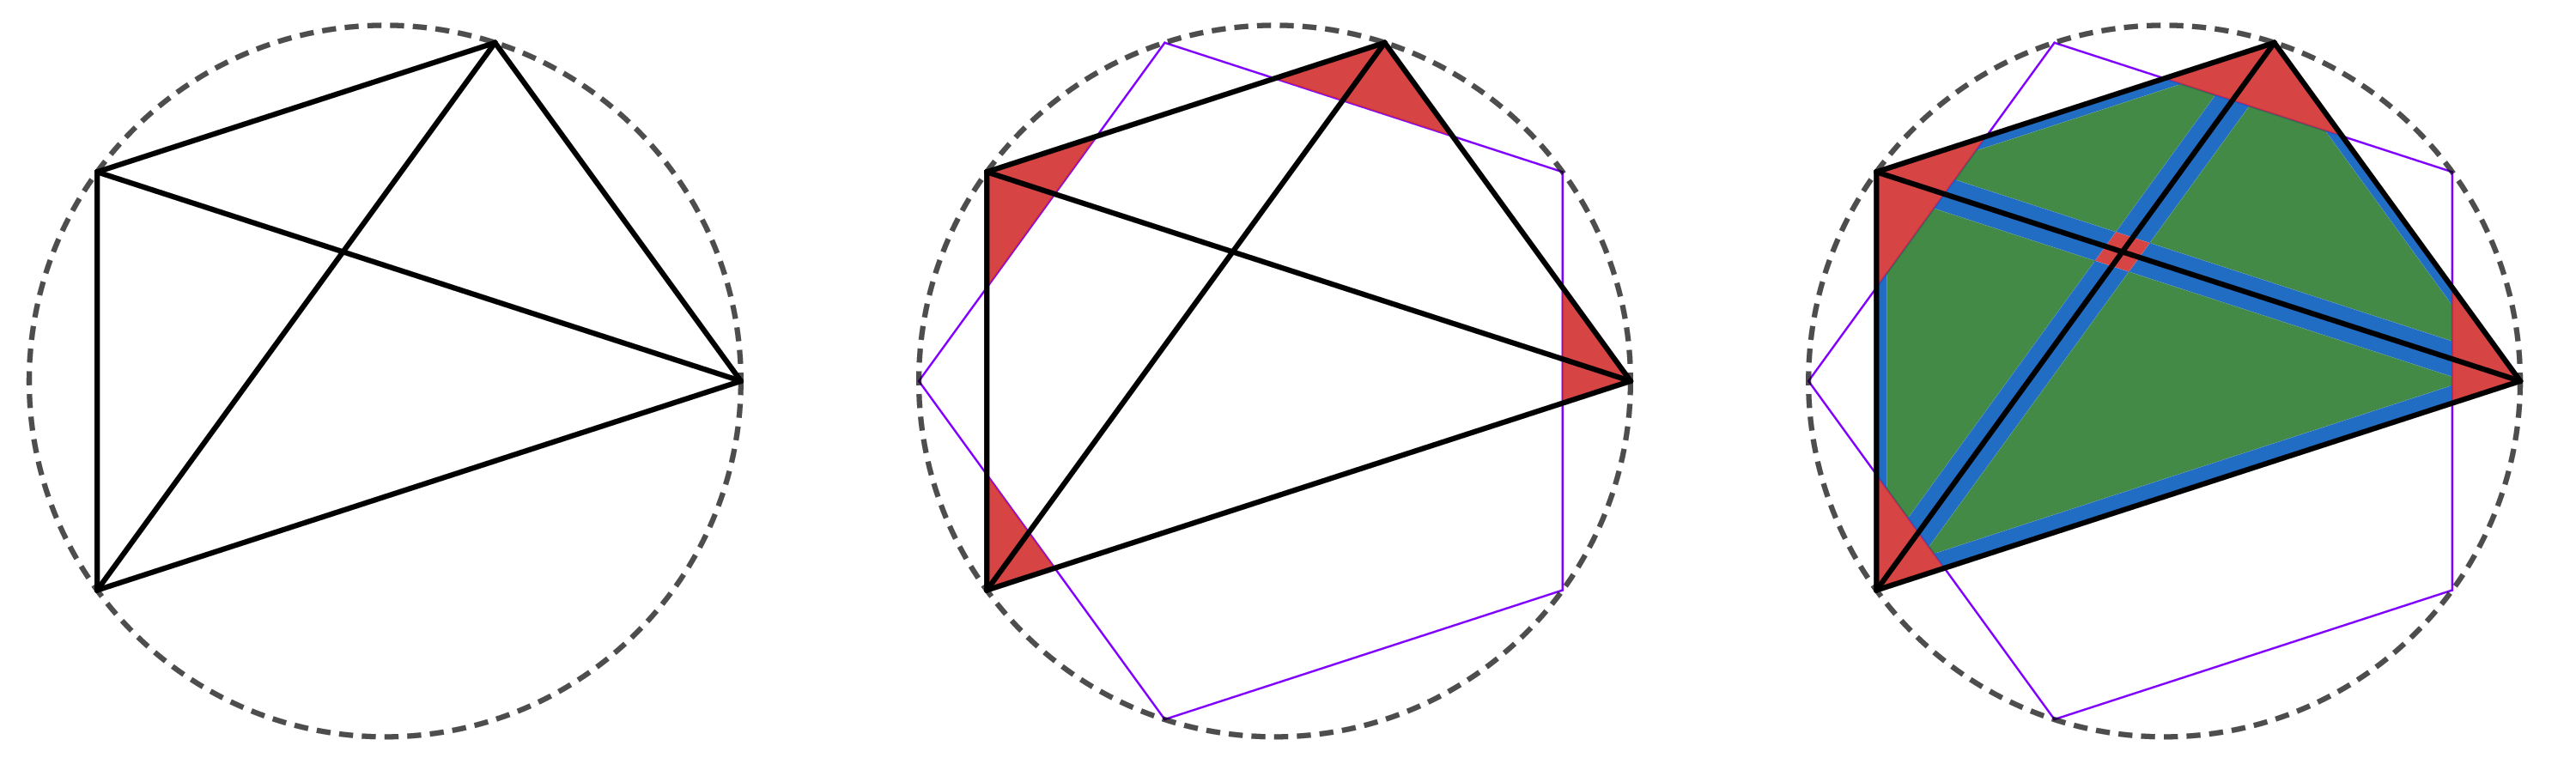
\includegraphics[width=0.9\textwidth]{figures/pl-segments.png}
	\caption{
		\textbf{The process of including additional segments into the plane to form piecewise-linear sleeves.}
		From left to right, we see first the image of the 1--skeleton of $N$ mapped to the plane, then the inclusion of the regular polygon $G_5$, which forms (red) vertex sleeves around the image of each vertex of $N$.
		The rightmost image depicts all sleeve segments as secants of $G_5$, forming the remaining (red) vertex sleeve, six (blue) edge sleeves, and four (green) face sleeves that subdivide $N$.
	}
	\label{fig:pl-segments}
\end{figure}


%\begin{figure}[h!]
%	\centering
%	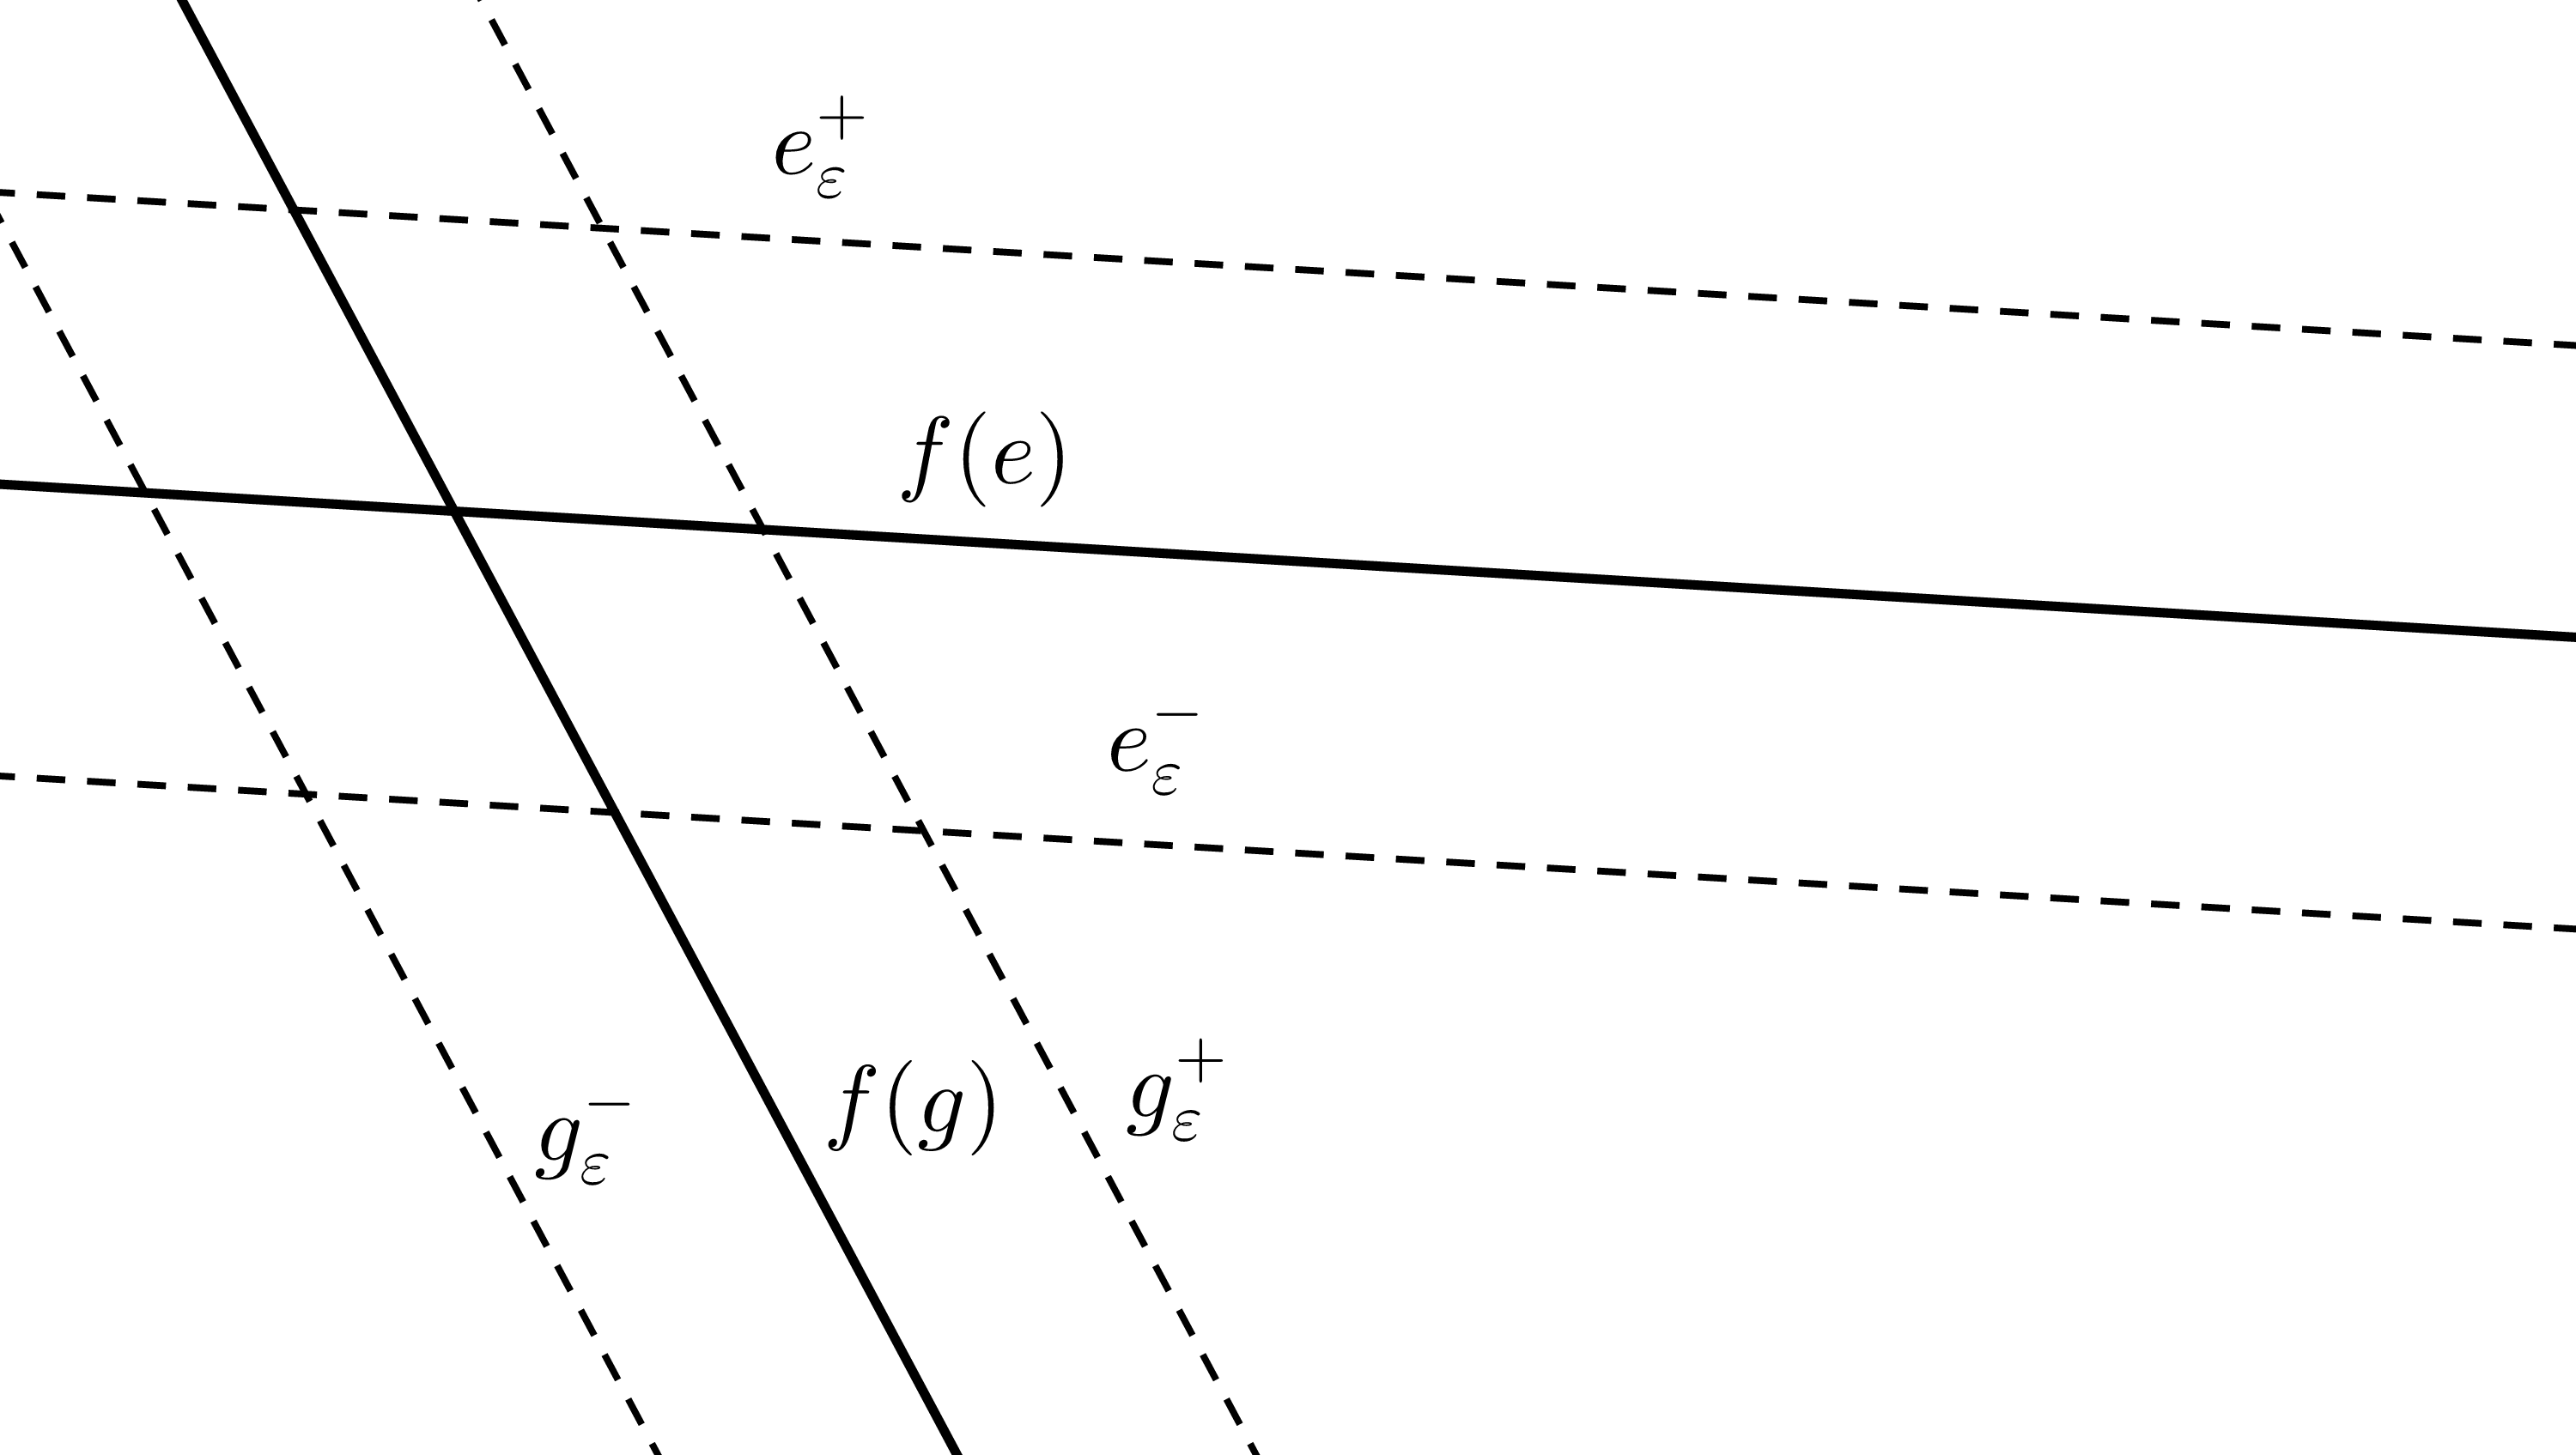
\includegraphics[width=0.9\textwidth]{figures/pl-sleeves.png}
%	\caption{
%		\textbf{A pair of sleeve segments in the plane.}
%		We show a pair of edges projections $f(e)$ and $f(g)$ in the plane, along with their associated sleeve segments.
%		Sleeve segments are necessary to ensure well-defined face, edge, and vertex block analogues in the subdivision of $N$.
%	}
%	\label{fig:pl-sleeves}
%\end{figure}
%
%\begin{figure}[h!]
%	\centering
%	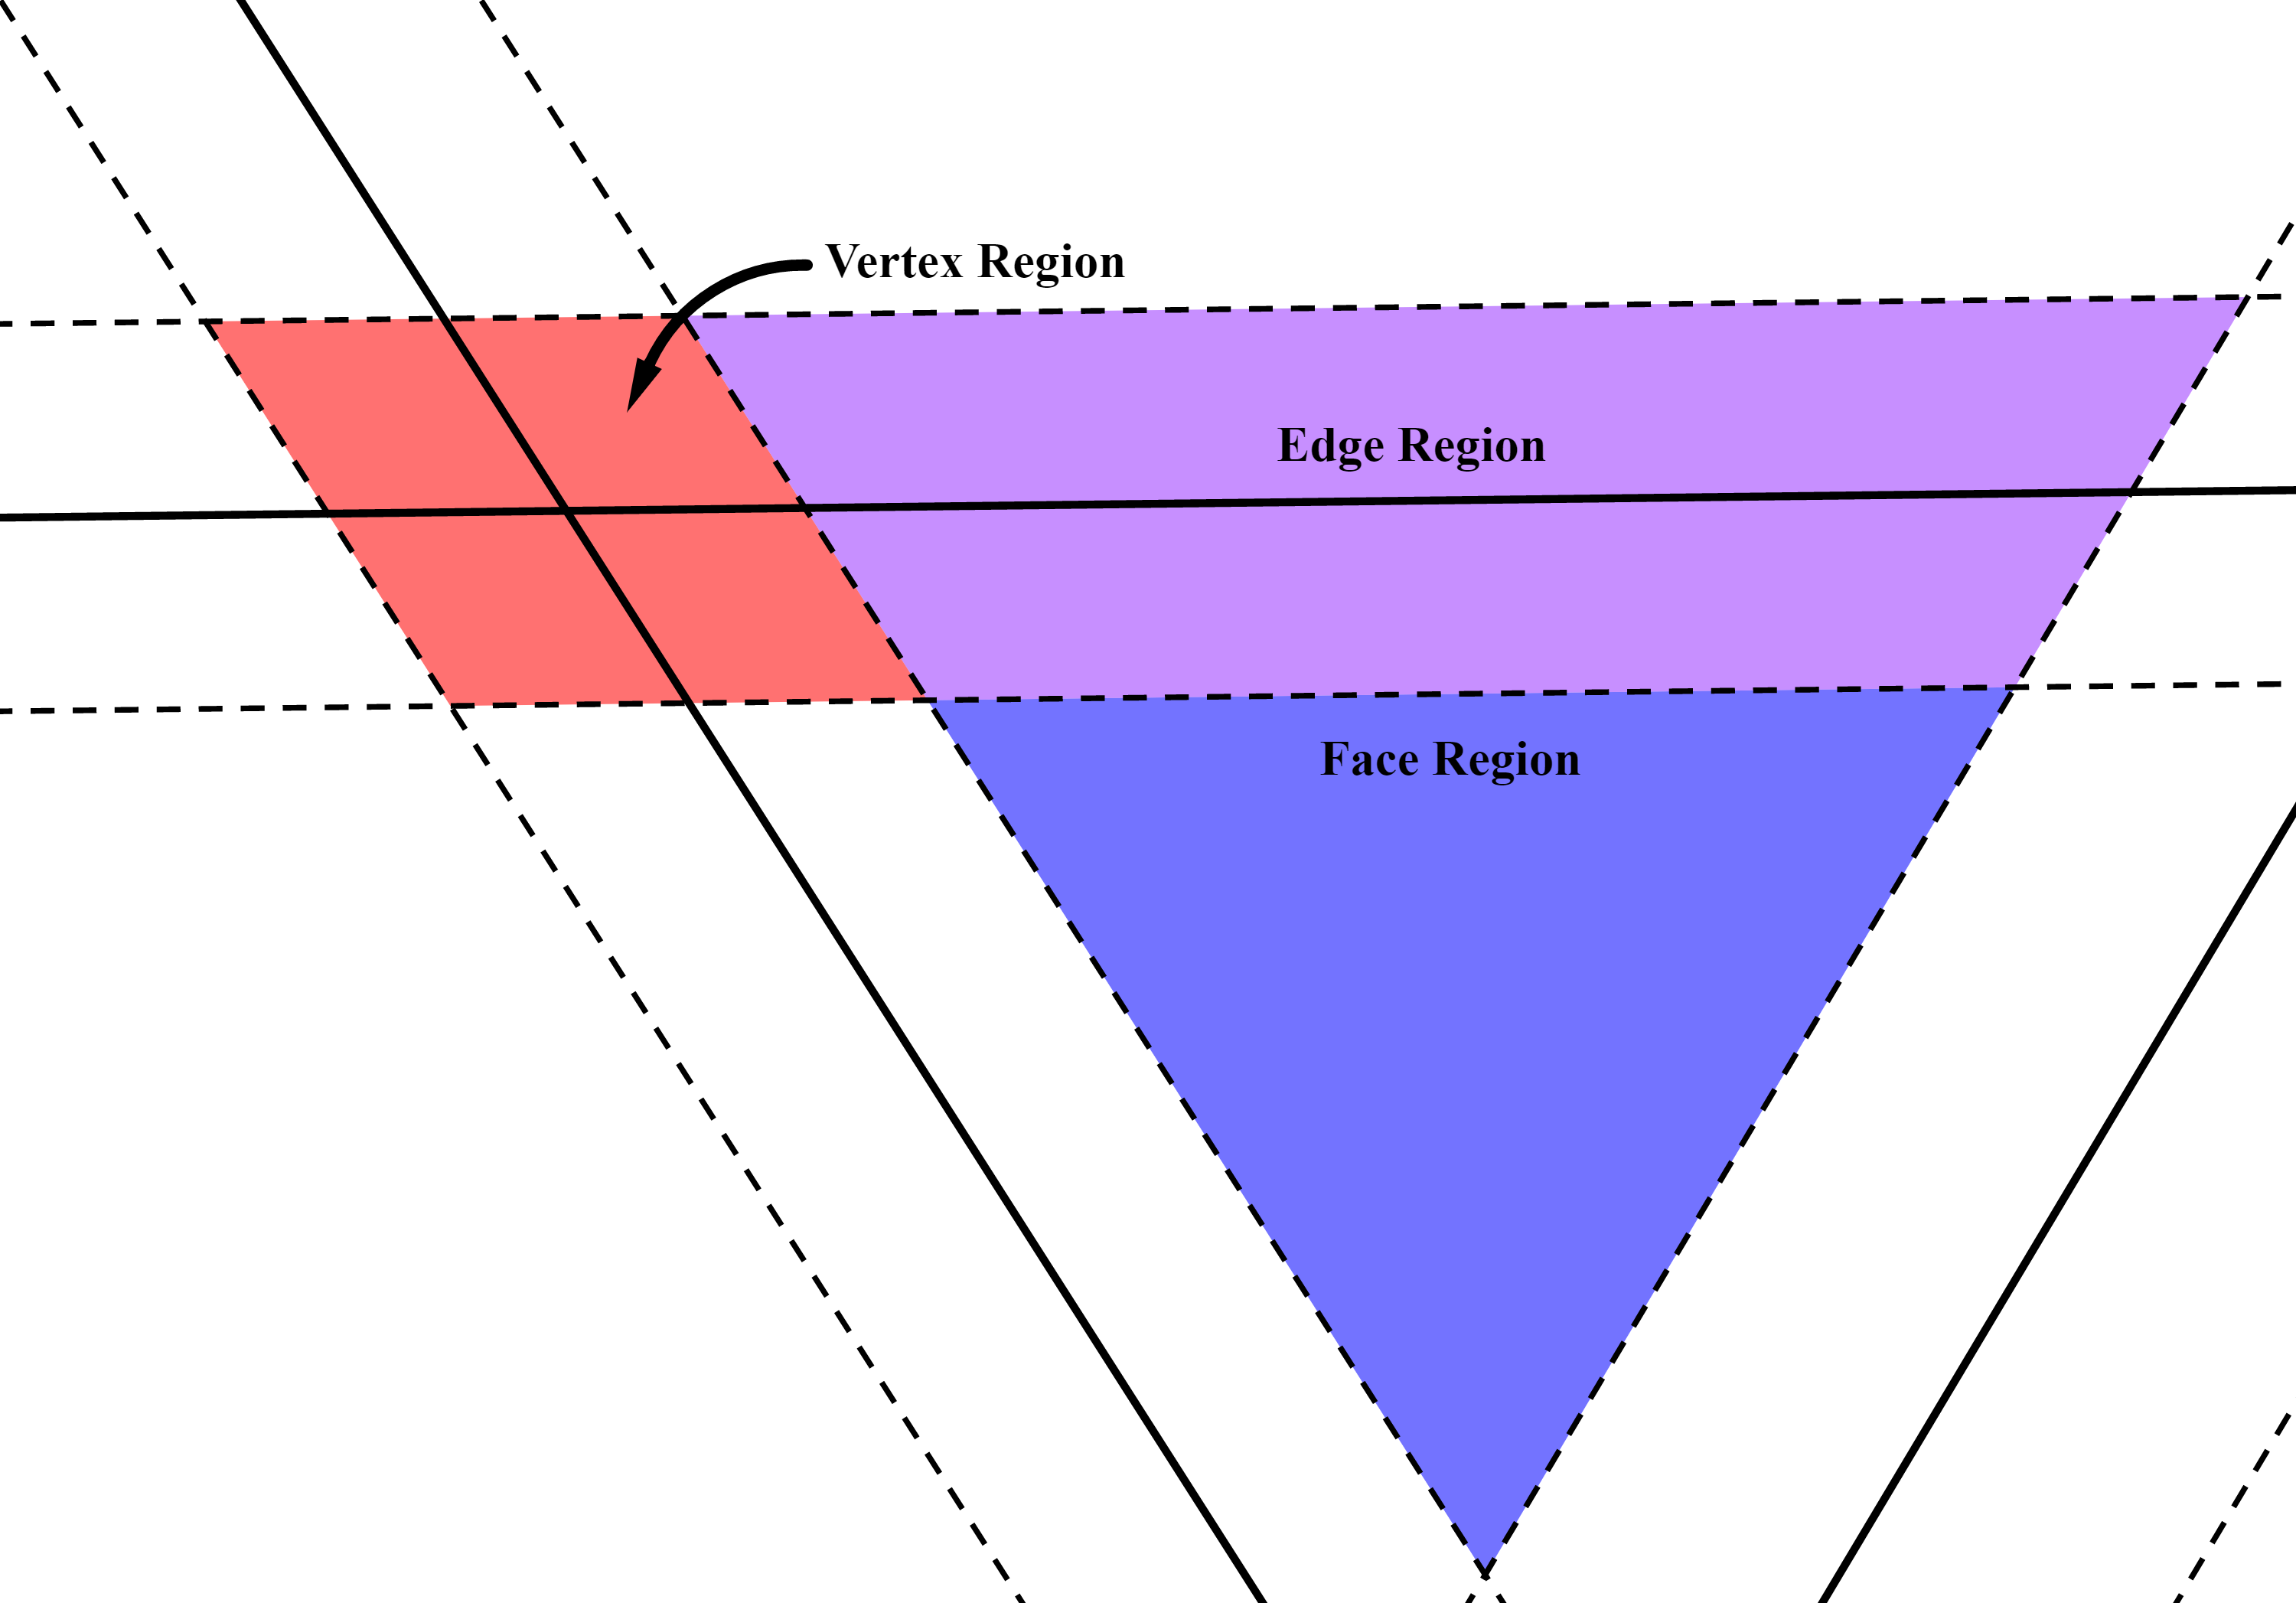
\includegraphics[width=0.9\textwidth]{figures/pl-regions.png}
%	\caption{
%		\textbf{Regions in the plane that correspond to combinatorial vertex, edge, and face block.}
%		The sleeve segments provide the same functionality as the sleeves in Chapter \ref{chapter:smooth}, in that the preimages of the regions they form behave similarly to the vertex, edge, and face blocks defined in Chapter \ref{chapter:smooth}.
%	}
%	\label{fig:pl-regions}
%\end{figure}

Take $L$ to be the set of line segments in the plane.
This consists of each segment of $G_k$, $f(e)$ for each $e\in N^1$, and the sleeve segments $e_\varepsilon^\pm$.
For each tetrahedron $\sigma$ of $N$, the polygons and intersections of $f\inv L\cap\sigma$ define a subdivision of $\sigma$ into a cell complex.
We implement this subdivision in Algorithm \ref{alg:subdividing-manifold} by constructing a new cell complex that is equivalent to $N$.
The subdivision iterates over all of the triangles and quads inside of $\sigma$, and the subdivision induced by a polygon is fully realized before moving on to the next.

For an example of subdivision, refer to Figure \ref{fig:standard-position-interior-exterior}, where a tetrahedron is being subdivided by an exterior triangle, an interior triangle, and an exterior quad.
We construct the subdivision of $\sigma$ as a 3--complex $\tau$, starting by setting $\tau = \sigma$.
Starting at the loop on line 6 of Algorithm \ref{alg:subdividing-manifold}, p. \pageref{alg:subdividing-manifold}, we'll assume that the brown segment that separates the pink vertex from the rest of $f(\sigma)$ is a segment from $G_k$ and set this segment as $l$.
This makes $\delta$ on line 7 the brown exterior triangle in $\sigma$.
Then the loop on line 8 runs over all 1--cells of $\tau$ that intersect the exterior triangle $\delta$ which are the three 1--cells of $\tau$ incident with the pink vertex.
We subdivide these 1--cells by their intersection with $\delta$, which amounts to including the corners of the $\delta$ exterior triangle into the complex, splitting the relevant 1--cells into a pair of 1--cells on either side of the corner.
This subdivision turns the three boundary triangles of $\tau$ that contained the pink vertex into pentagons.
We move to the loop on line 12, where we subdivide these three boundary pentagons by the three triangular edges of $\delta$.
Each pentagon is subdivided into a triangle and a quadrilateral.
Finally, in the loop at line 16 we subdivide the only 3--cell of $\tau$ into a tetrahedron containing the pink vertex and a triangular cylinder away from the pink vertex.

Heading back to the top of the loop at line 6 and assuming we have exhausted all segments of $G_k$, we may now consider any segment.
Setting $l$ to be the blue interior edge of Figure \ref{fig:standard-position-interior-exterior} makes $\delta$ the blue interior triangle.
Moving through the loop at line 8, we find
\begin{enumerate}
	\item the intersection of $\delta$ with the 1--cell of $\tau$ containing the blue and red vertices and 
	\item the intersection of $\delta$ with the brown exterior triangle located on the shared boundary of the pair of 2--cells in $\pd\tau$ induced by the subdivision of the 2--cell in $\pd\sigma$ opposite the green vertex.
\end{enumerate}
We then insert 0--cells into $\tau$ at these intersections, subdividing 1--cells as necessary.
The loop at line 12 now runs over the intersections of $\delta$ with the 2--cells of $\tau$, and these intersections occur with the triangle in $\pd\tau$ opposite the pink vertex and with the 2--cells in $\pd\tau$ induced by the subdivision of the 2--cell in $\pd\sigma$ opposite the green vertex.
We add 1--cells to $\tau$ that divide the quadrilateral into a pair of quadrilaterals and the triangles into pairs of triangles.
Finally, the loop at line 16 subdivides both 3--cells of $\tau$, splitting them each in half as polyhedrons.
It is left to the reader to continue the subdivision of $\tau$ in Figure \ref{fig:standard-position-interior-exterior}, where the remaining exterior quad subdivides five 1--cells, five 2--cells, and two 3--cells.

Observe also that the gluing defined on the tetrahedra of $N$ is used to produce $M$ as well.
To see this, let $\sigma$ and $\sigma'$ be tetrahedra of $N$ that are glued together over a triangular face, $\Delta\in\sigma$ and $\Delta'\in\sigma'$.
Then Algorithm \ref{alg:subdividing-manifold} produces a pair of 3--complexes $\tau$ and $\tau'$, and $\Delta$, $\Delta'$ are each subdivided into boundary 2-complexes of $\tau$ and $\tau'$.
These subdivisions are induced by the subdivisions of $f(\Delta)$ and $f(\Delta')$ in the plane but, because $\Delta$ and $\Delta'$ are identified in the gluing of $N$, $f(\Delta)=f(\Delta')$ and the subdivisions of $\Delta$ and $\Delta'$ are equivalent.
The gluing that defines $M$ is therefore constructed by subdividing the gluing that defined $N$.

\begin{algorithm}[h!]
	\caption{Using a subdividing map to subdivide the input 3--manifold triangulation}
	\label{alg:subdividing-manifold}
	\KwData{A closed, orientable 3--manifold triangulation $N$ with subdividing map $f:N\to\RR$}
	\KwResult{A closed, orientable 3--dimensional cell complex $M$ that is a subdivision of $N$}
	\Begin{
%		$k = $ the smallest odd number greater than or equal to $|N^0|$\;
%		$G_k = $ the secants of the regular $k$-gon inscribed in the circle with one corner at $(-1,0)$\;
		$L = G_k\cup\{f(e)\;|\;e\in N^1\}\cup\{e_\varepsilon^\pm\;|\;e\in N^1\}$\;
		\ForEach{tetrahedron $\sigma$ of $N^3$}{
			We construct a 3--dimensional cell complex $\tau$ that is the subdivision of $\sigma$ prescribed by $f$\;
			$\tau = \sigma$\;			
			\ForEach{segment $l$ in $L$ such that $l\cap f(\sigma)\neq\emptyset$ and $l\nsubseteq \pd f(\sigma)$, iterating over the segments of $G_k$ first}{
				$\delta = $ the intersection of $\sigma$ with $f\inv l$\;
				\ForEach{intersection $d_0 \in\delta\cap\tau^1$ such that $d_0\notin \tau^1$}{
					$d_0 = \delta\cap t_1$ for some 1--cell $t_1$ of $\tau$\;
					Subdivide $t_1$ by $d_0$ into a pair of 1--cells $td_1$ and $dt_1$\;
				}
				\ForEach{intersection $d_1\in\delta\cap\tau^2$}{
					$d_1 = \delta\cap t_2$ for some 2--cell $t_2$ of $\tau$\;
					Subdivide $t_2$ by $d_1$ into a pair of 2--cells $td_2$ and $dt_2$\;
				}
				\ForEach{intersection $d_2\in\delta\cap\tau^3$}{
					$d_2 = \delta\cap t_3$ for some 3--cell $t_3$ of $\tau$\;
					Subdivide $t_3$ by $d_2$ into a pair of 3--cells $td_3$ and $dt_3$\;
				}
			}
		}
		$M = $ the set of 3--complexes $\tau$ constructed above, glued together as prescribed by the gluing maps of $N$ and the identification of the $\tau$ as subdivisions of the tetrahedra of $N$\;
	}
\end{algorithm}


We subdivided $N$ into $M$ in order to identify analogues to the face, edge, and vertex blocks of Chapter \ref{chapter:smooth}.
The analogous blocks are defined exactly as they were in Chapter \ref{chapter:smooth} --- the sleeve segments subdivide the plane into regions homeomorphic to disks, those disks are classified by whether they contain a crossing of $f(N^1)$, intersect $f(N^1)$ but do not contain a crossing, or do not intersect $f(N^1)$ at all.
The preimage of a region that contains a crossing is a \emph{combinatorial vertex block}, the preimage of a region that intersects $f(N^1)$ but does not contain a crossing is a \emph{combinatorial edge block}, and the preimage of a region that is disjoint from $f(N^1)$ is a \emph{combinatorial face block}.
Symmetric names are used for the regions that these blocks project onto --- combinatorial face (resp. edge, vertex) blocks map through $f$ to \emph{combinatorial face (}resp. \emph{edge, vertex) regions}.
Figure \ref{fig:pl-segments} illustrates the regions in the plane that produce such blocks.
These preimages exhaust the cells of $M$, providing a decomposition into subcomplexes.
This decomposition is not a partition --- some cells are assigned to more than one block.
Such an assignment happens precisely when a cell is mapped through $f$ to the shared boundary of different combinatorial regions.

%Note: we 'need' to include S^1\in\RR to actually form the regions discussed, but that's pretty obvious so we won't address it unless requested.

Algorithm \ref{alg:subdividing-manifold} produces a cell complex $M$ that is a polyhedral gluing, and we would prefer to replace $M$ with an equivalent triangulation.
This is done by first replacing each polyhedron $P$ that is not a tetrahedron with the cone on $\pd P$.
At each polyhedron $P$ this replaces the single 3--cell interior of $P$ with $|P^2|$ new polyhedra, each of which has at most one non-triangular face.
Because $M$ is closed, that face is glued to another face of the same polygonal type.
If $P,Q$ are a pair of polyhedra of $M$ that are glued over the faces $P_i^2$ and $Q_j^2$, each of which is a $k$--gon, $k>3$, then we further subdivide $P_i^2\sim Q_j^2$ into $k-2$ triangles, and replace the newly introduced polyhedra with $k-2$ new tetrahedra, as illustrated in Figure \ref{fig:subdivide-polyhedra}.
This process thus adds $2k-4$ tetrahedra per $k$--gon 2--cell of $M$, $k>3$.
Note that if the boundary of $P$ and $Q$ is not essential, i.e.\ is not contained in the boundary of some combinatorial block, then we can instead replace the polyhedra incident to that face with the more efficient (when $k>4$) triangulation of the suspension of the $k$--gon with $k$ tetrahedra, also illustrated in Figure \ref{fig:subdivide-polyhedra}.

\begin{figure}[h!]
	\centering
	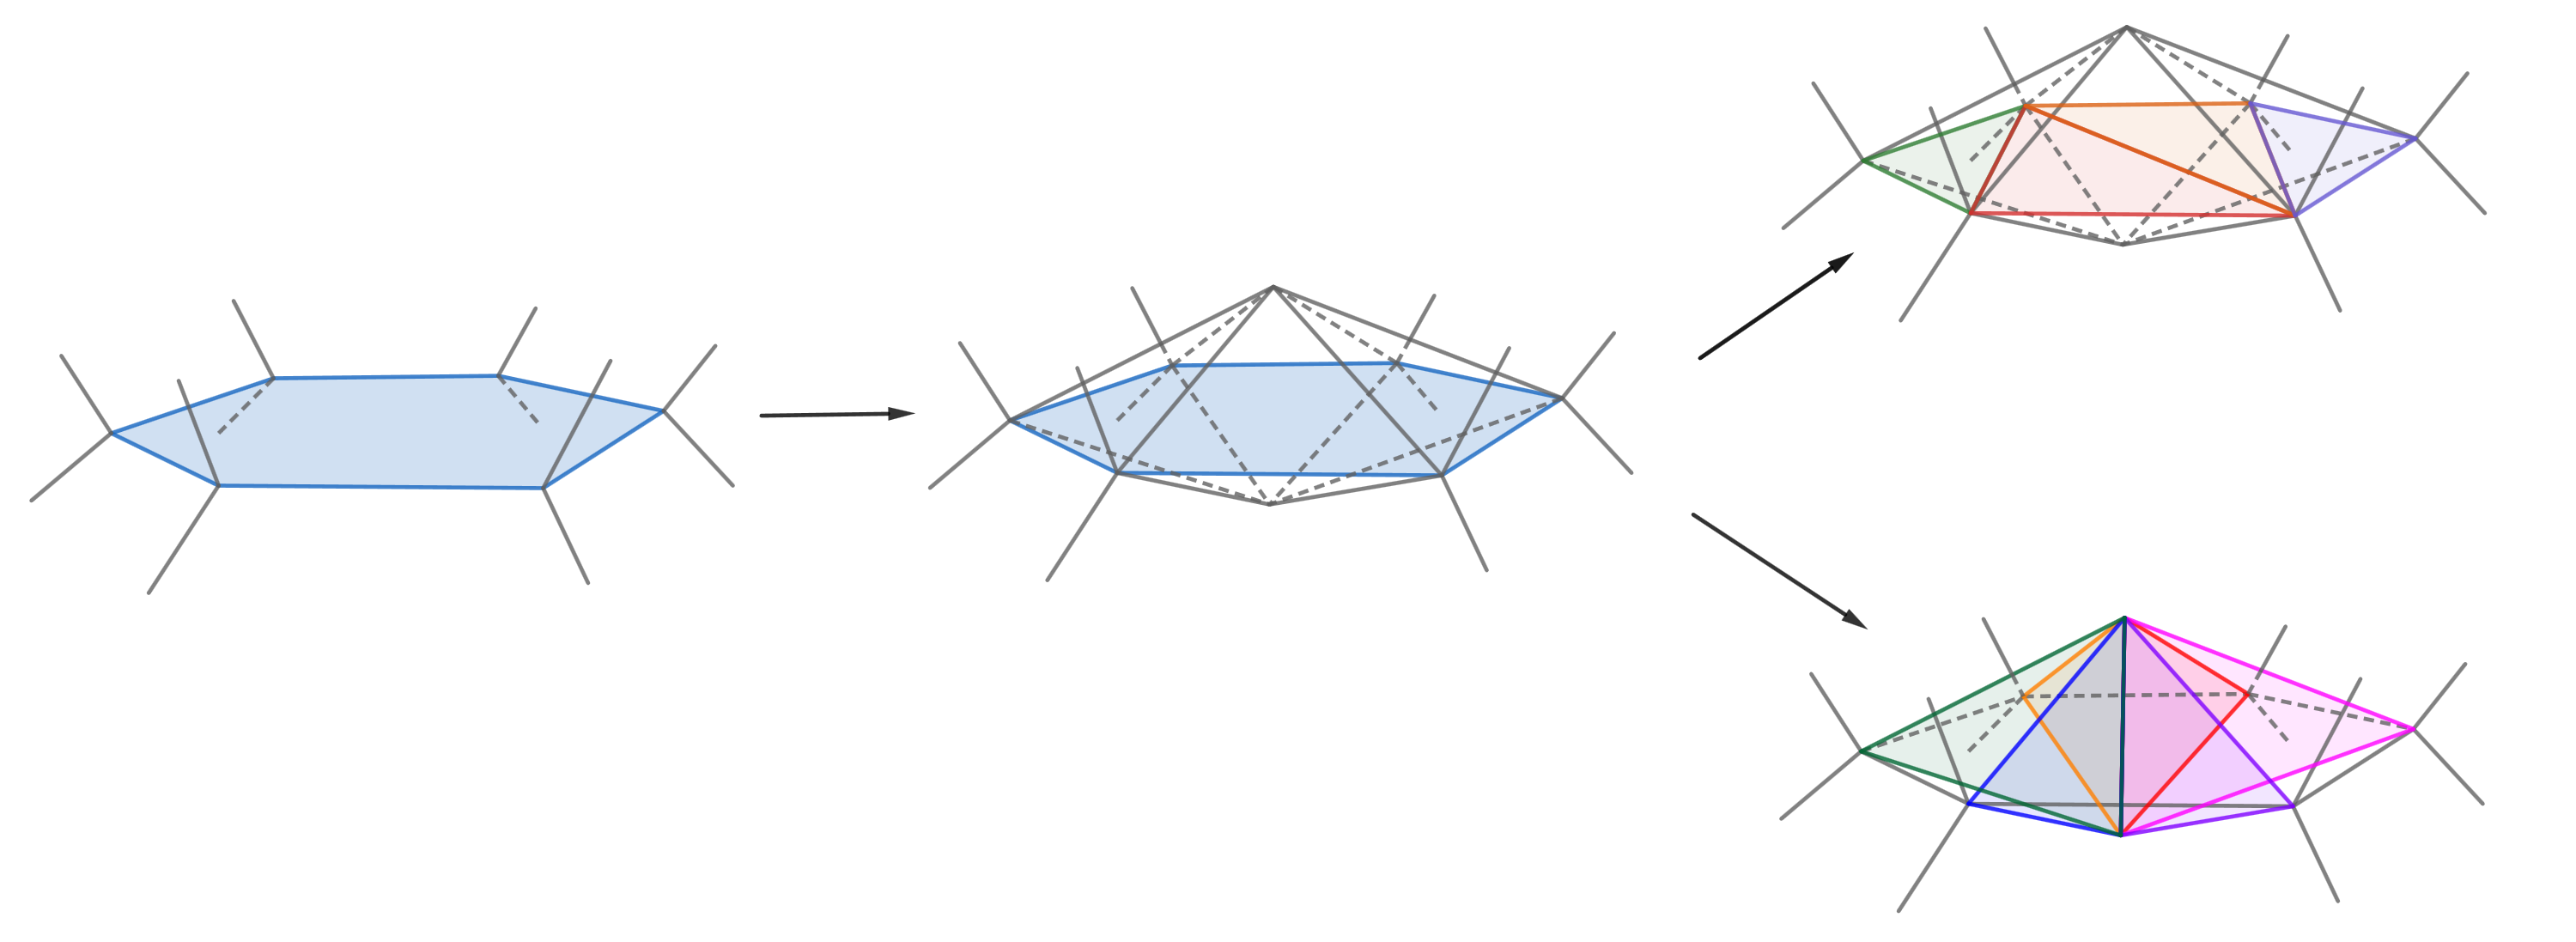
\includegraphics[width=0.9\textwidth]{figures/subdivide-polyhedra.png}
	\caption{
		\textbf{Subdividing polyhedral cells.}
		From left to right, we see first the polygonal boundary 2--cell between a pair of polyhedral cells.
		Next, the polyhedral cells are subdivided by replacing them with the cone of their boundaries.
		Finally, either the polyhedra on each side of the polygon are subdivided into reflection-identical triangulations or the pair is replaced by a $k$ simplex triangulation  of the suspended $k$--gon.
	}
	\label{fig:subdivide-polyhedra}
\end{figure}


Next, we form the 4--thickening $W=M\times\Ilit$.
This is done by attaching triangulated 4--prisms to each tetrahedron of $M$, where a triangulated 4--prism is the 4--dimensional extension of the triangulated 3--prism described in Theorem 3.1 of \cite{burton2011simplification}.
Specifically, the $(n+1)$-prism triangulation is constructed as the cone of the triangulated $n$--sphere whose `top' and `bottom' are $n$--simplices and whose `sides' are the triangulated $n$--prism, where the triangulated 1--prism is a single edge connecting a pair of vertices.
Triangulated 1--, 2--, and 3--prisms are illustrated in Figure \ref{fig:prisms}.
We use prisms at this stage because the `walls' of the prisms are identical, making the gluing of prisms automatic.
Denoting the number of $n$--simplices used to triangulate the $n$--prism by $p(n)$, and setting $p(1)=1$, we find that
\[
	p(n) = 2 + n\cdot p(n-1)
\]
due to the recursive nature of prism construction.
This means a 2--prism is triangulated with 4 triangles, a 3--prism with 14 tetrahedra, and a 4--prism with 58 pentachora.

\begin{figure}[h!]
	\centering
	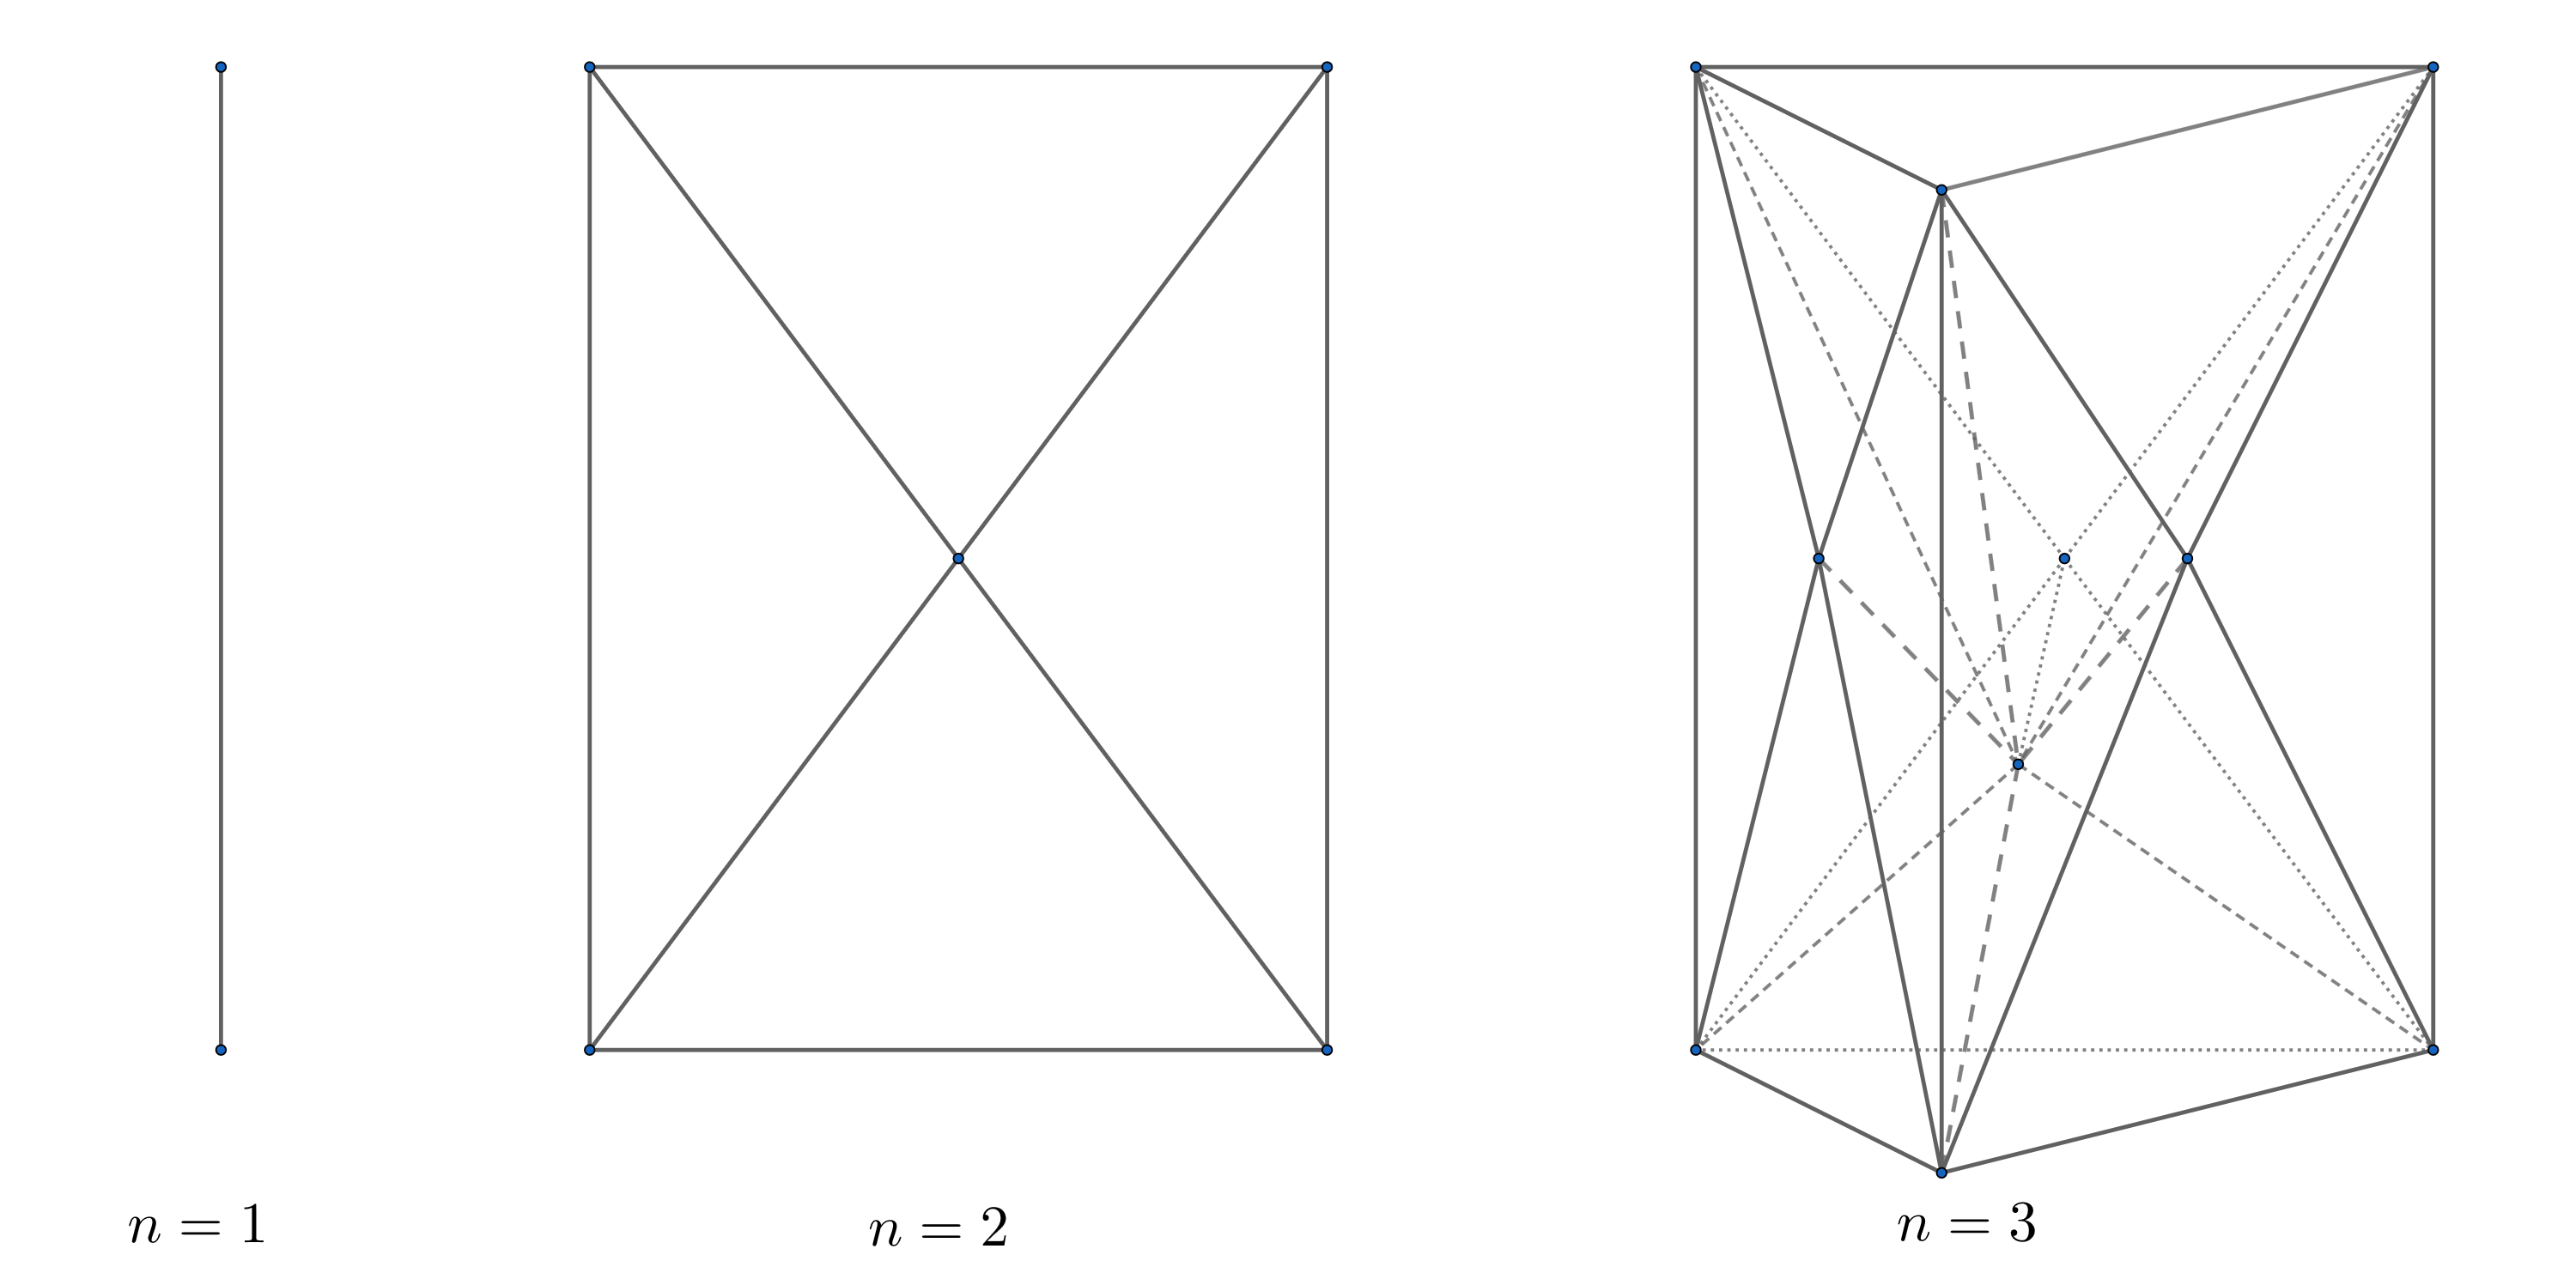
\includegraphics[width=0.9\textwidth]{figures/prisms.png}
	\caption{
		\textbf{The first three triangulated prisms.}
		From left to right, we see the triangulated prisms with identical walls in dimensions 1, 2, and 3.
	}
	\label{fig:prisms}
\end{figure}

Finally, we examine how the smooth singularity theory is adapted by examining our combinatorial blocks.
As in the smooth case, a combinatorial face block is a triangulated solid torus, a combinatorial edge block has the structure of an interval crossed with a triangulated surface that projects over a small transversal to the corresponding edge sleeve, and a combinatorial vertex block has the structure of a regular neighbourhood of the 1--dimensional subcomplex over its planar vertex.
For combinatorial vertex blocks, this amounts to being a (3,1)--handlebody and this handlebody is determined by how its boundary surface is constructed.
However, this boundary surface is the union of subtriangulations of combinatorial edge block boundaries, and these subtriangulations are precisely the surfaces that project over small transversals to the edge sleeve, making these surfaces perhaps the most topologically interesting structure in our construction.



Each edge $e$ of $N$ is mapped to a secant of circle, splitting the disc into exactly 2 sectors: the `left' and `right' sides of $f(e)$.
Denote the set of tetrahedra of $N$ containing $e$ by $\del$.
Each tetrahedron $\sigma$ of  $\del$ is either mapped to the left of $e$, to the right of $e$, or across $e$ based on the image of the edge in $\sigma$ opposite $e$.

First, we consider the situation when all of the tetrahedra containing $e$ are mapped to the same side of $f(e)$.
This happens, for example, when $f(e)$ is on the boundary of $f(N)$ and in this situation $e$ is analogous to a definite fold.
Let $\gamma$ be the boundary between an edge sleeve around a section of $e$ and an adjacent vertex sleeve.
Then $\gamma$ is a short interval transverse to $e$ and we show that the preimage of $\gamma$ in $\del$ is a triangulated 2--disc.

The interval is triangulated with two edges and three vertices: one vertex at each of the sleeve segments around $f(e)$ and one vertex on $f(e)$.
We'll call these vertices $x,y,z$, letting $x$ be the vertex on the side of $e$ that $\del$ is mapped to and $y$ the vertex on $f(e)$.
In $M$, our subdivision of $N$, $f\inv(x)\cap\del$ is a triangulated circle, $f\inv(y)\cap\del$ is a single vertex, and $f\inv(z)\cap\del$ is empty.
The preimage of the edge $[x,y]$ in $\gamma$ forms the triangles that complete the 2--disc we expected to find, illustrated in Figure \ref{fig:pl-definite-fold}.

\begin{figure}[h!]
	\centering
	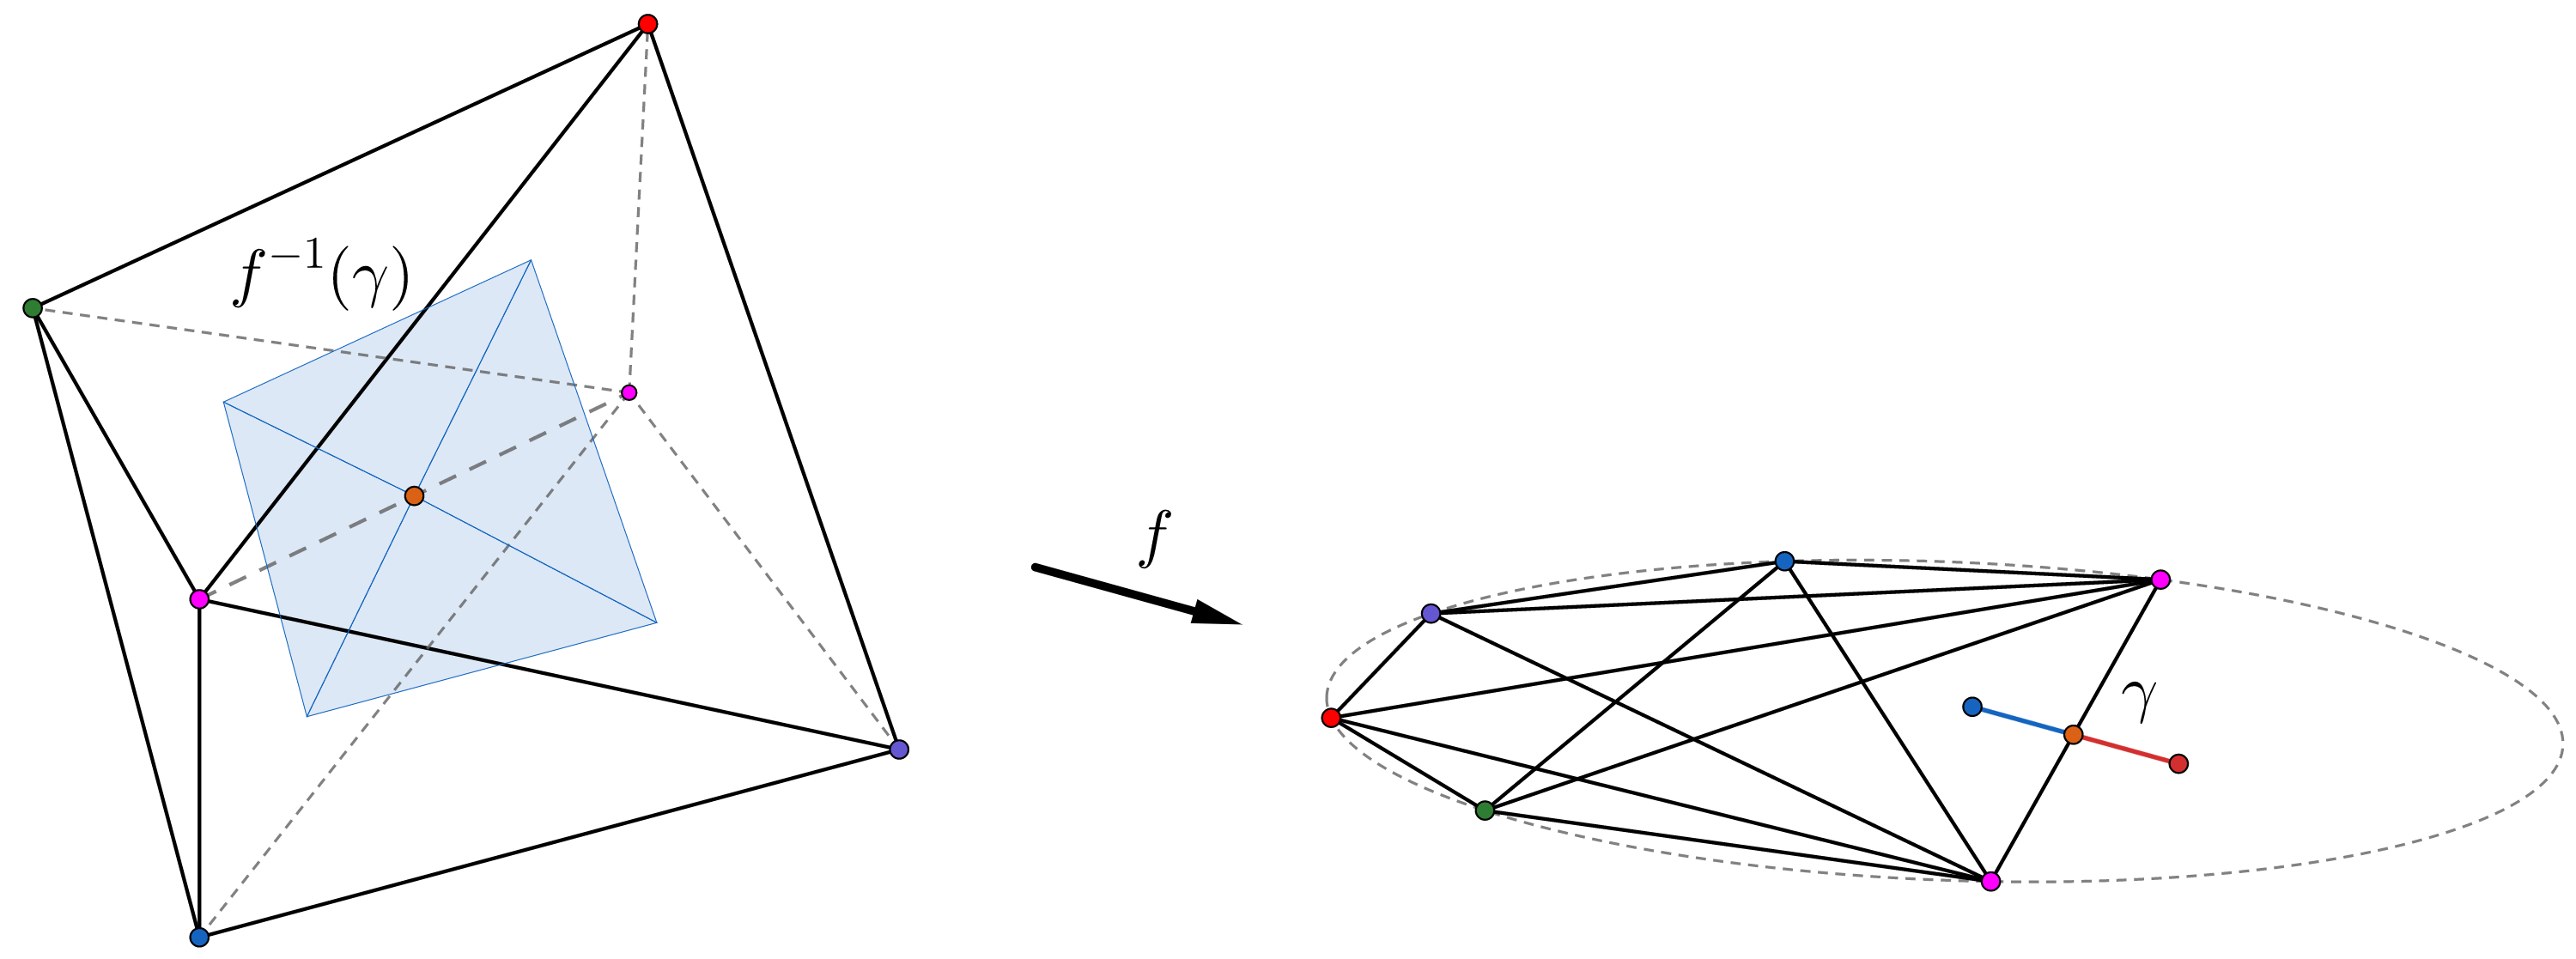
\includegraphics[width=0.9\textwidth]{figures/pl-definite-fold.png}
	\caption{
		\textbf{An edge link and its image through a subdividing map.}
		We see the 2--disc triangulation, where the preimage of the boundary point of $\gamma$ in the image of $f$ is a single triangulated circle and that circle is wholly contained in the tetrahedra incident to the edge $\gamma$ transverses.
	}
	\label{fig:pl-definite-fold}
\end{figure}

Next, what happens when a tetrahedron of $\del$ is mapped across $f(e)$?
Because $N$ is closed, the number of tetrahedron in $\del$ that map across $f(e)$ is always even.
The tetrahedra of $\del$ have a circular order defined by edges in $\del$ that are opposite $e$, and all tetrahedra between a crossing pair are mapped to the same side of $f(e)$.
When the number of crossing pairs is exactly one, we have a situation analogous to that of the regular edge block.
The tetrahedra of $\del$ that map to one side of $f(e)$ each contribute a single triangle to the surface $f\inv(\gamma)$, and the tetrahedra that map across $f(e)$ cause the disc that is $f\inv(\gamma)\cap\del$ to lie incident to the boundary of $\del$, as depicted in Figure \ref{fig:pl-regular-surface}.
This boundary portion of $f\inv(\gamma)\cap\del$ is a pair of (2,1)--handle attachment sites, but because there are only two sides of $f(e)$ in the disc the handle is attached in an orientation preserving way.

\begin{figure}[h!]
	\centering
	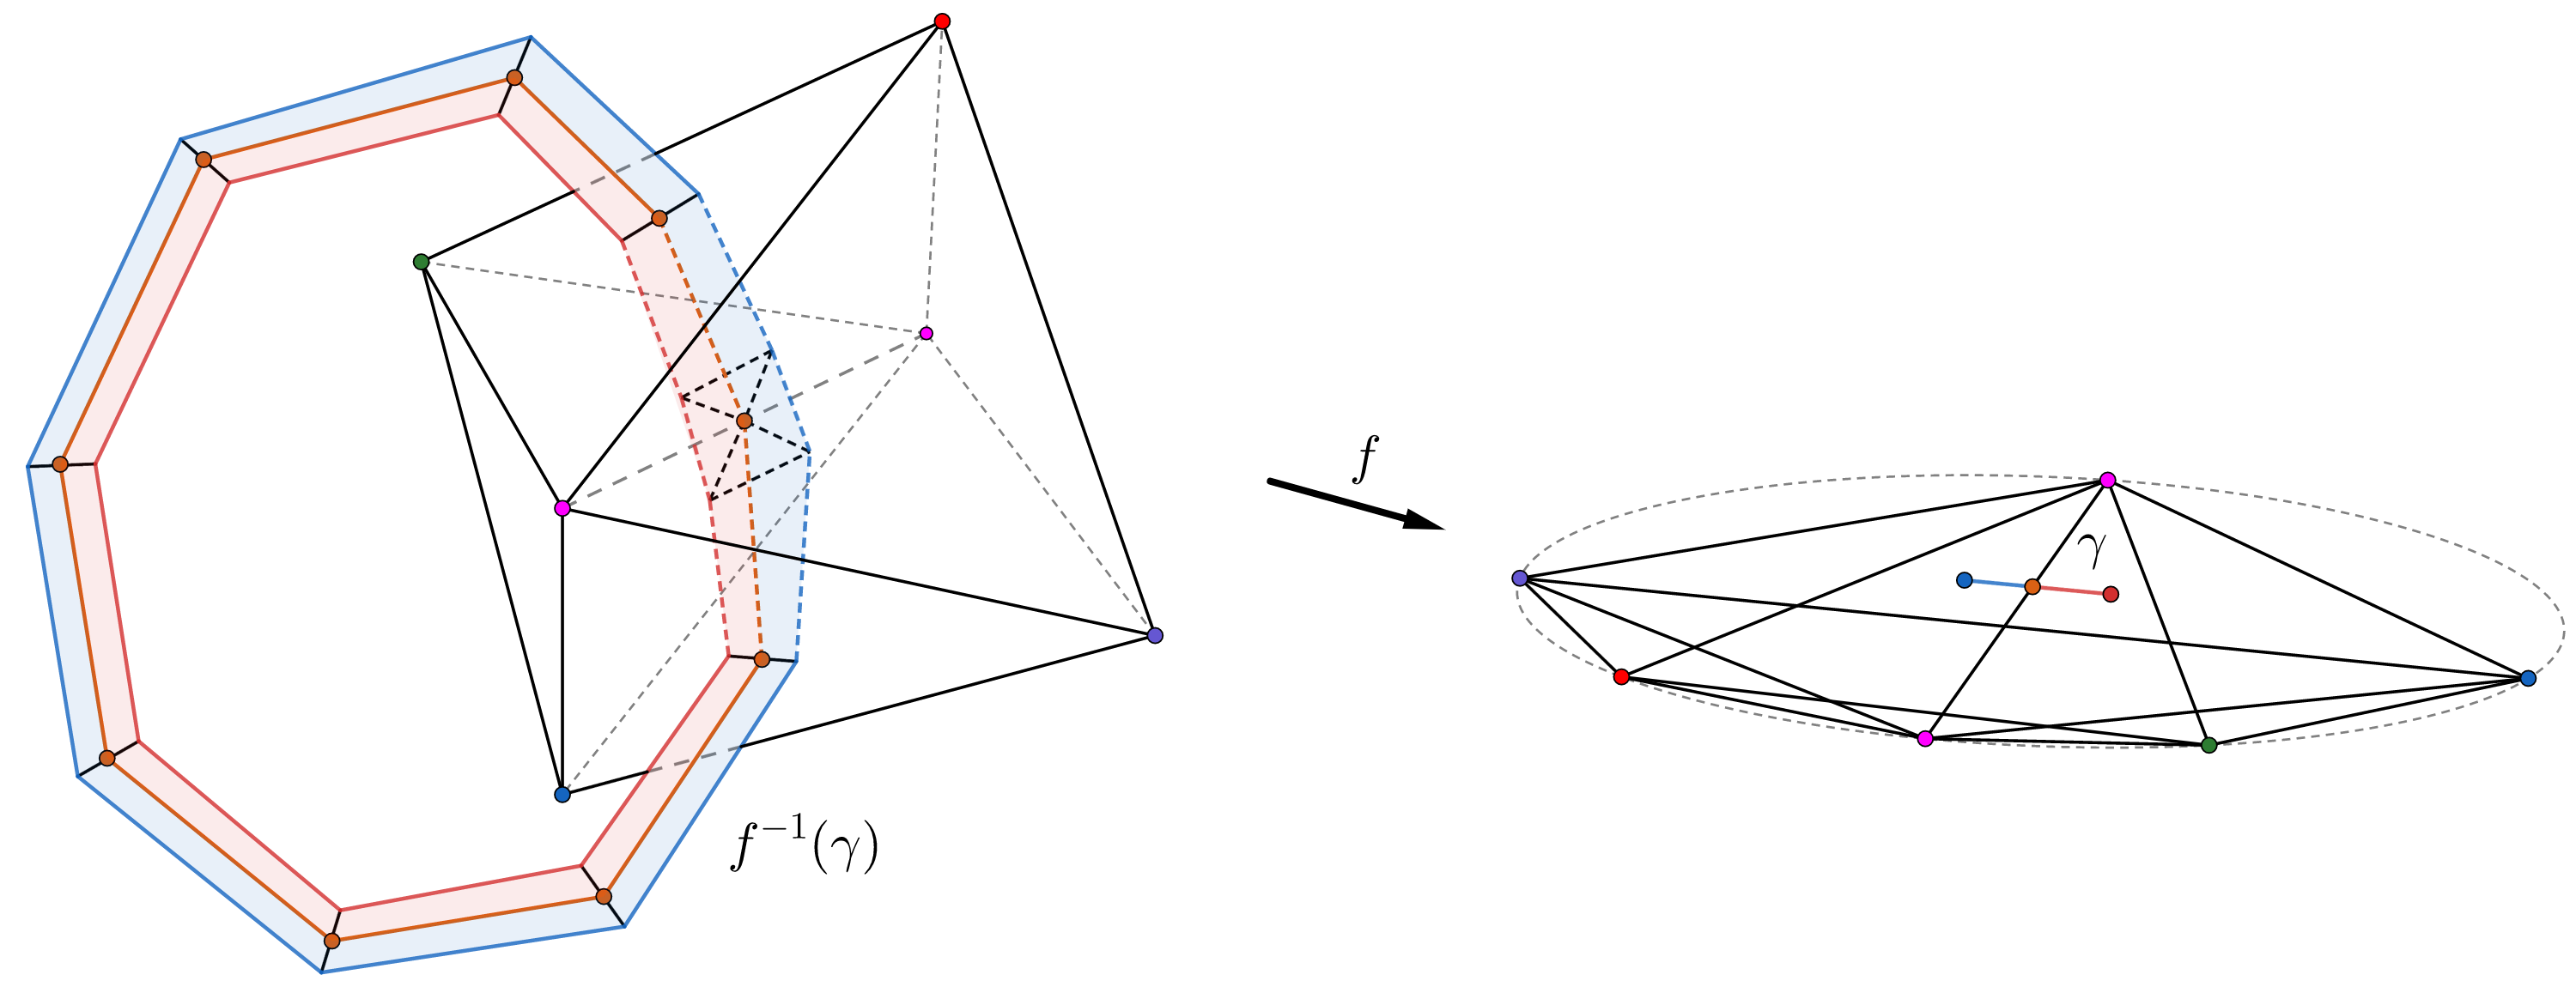
\includegraphics[width=0.9\textwidth]{figures/pl-regular-surface.png}
	\caption{
		\textbf{A transversal surface around an edge $e$ when exactly one pair of tetrahedra map across $f(e)$.}
		The transversal $\gamma$ has two halves, one on either side of $f(e)$.
		Lifted to $N$, $f\inv(\gamma)\cap\del$ is a disc incident to $\pd\del$ in exactly two (2,1)--handle attachment sites, and the (2,1)--handle attachment is orientation preserving.
	}
	\label{fig:pl-regular-surface}
\end{figure}

When multiple tetrahedra of $\del$ map across $f(e)$, the idea generalizes.
If $2n$ such tetrahedra map across $f(e)$, then there are $2n$ (2,1)--handle attachment sites in $f\inv(\gamma)\cap\pd\del$, these handles are attached in an orientation preserving way, and the pairing of attachment sites depends on the topology of $N$ outside of $\del$.
Figure \ref{fig:pl-indefinite-fold} shows a possible resolution of the case $2n=4$, where we always obtain a pair-of-pants surface (note that the only handle attachments that would not produce a pants surface are not orientation preserving).
Moreover, every surface in the disjoint collection of surfaces $f\inv(\gamma)$ is a (multiply) punctured 2--sphere.
The surface of $f\inv(\gamma)$ that intersects $\del$ is an $(n+1)$--punctured 2--sphere, and all other surfaces are twice-punctured (i.e. annuli).

\begin{figure}[h!]
	\centering
	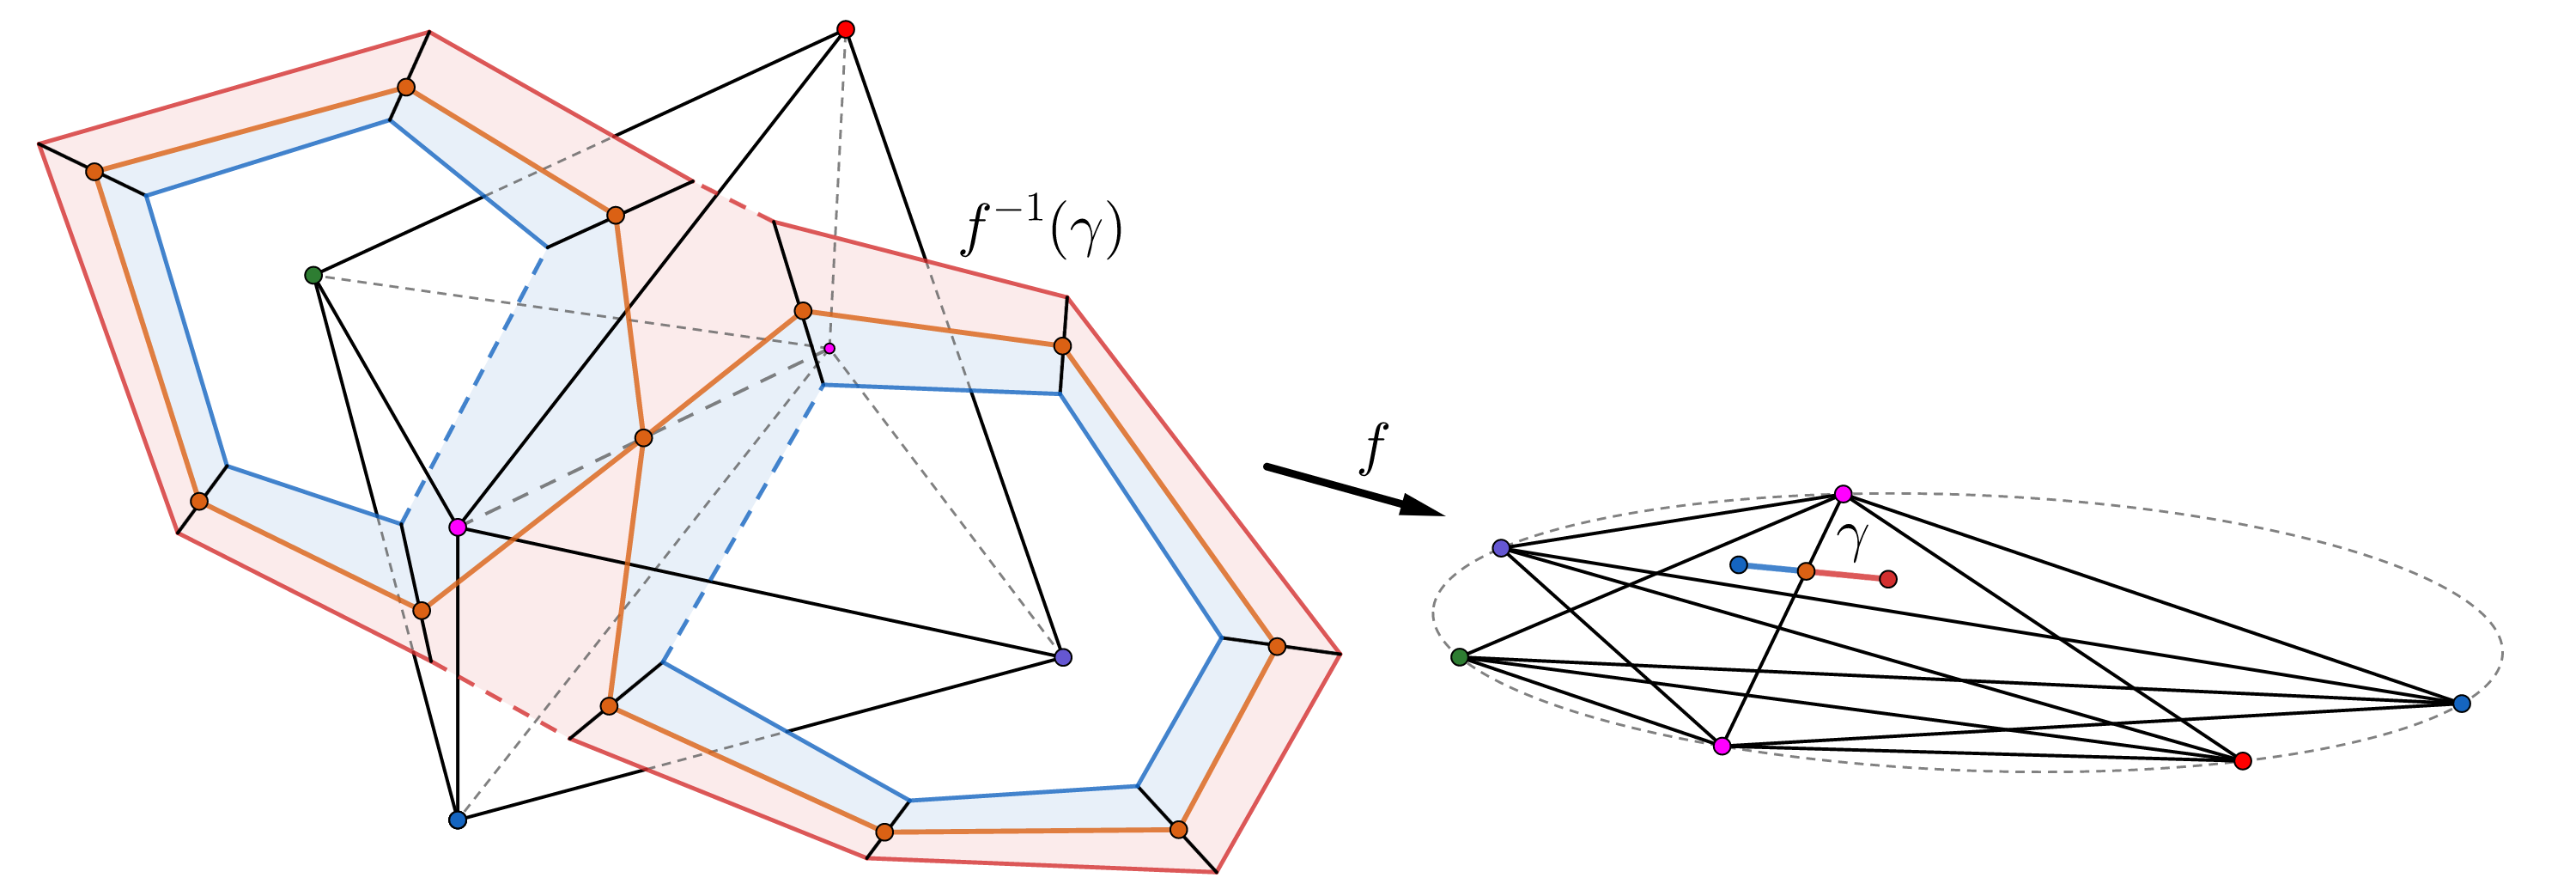
\includegraphics[width=0.9\textwidth]{figures/pl-indefinite-fold.png}
	\caption{
		\textbf{A transversal surface around an edge $e$ when exactly two pairs of tetrahedra map across $f(e)$.}
		When two pairs of tetrahedra map across $f(e)$ we find two pairs of (2,1)--handle attachment sites and the handle attachment is still orientation preserving.
		The pairing of attachment sites is determined by the structure of $N$: the (2,1)--handle attachments could be different in $N$, with the sites near the red and blue vertices being connected rather than the green and purple sites as depicted in the figure.
		However, the identification of sites across the disc $f\inv(\gamma)\cap\del$ is not possible because such a handle attachment would not be orientation preserving.
	}
	\label{fig:pl-indefinite-fold}
\end{figure}

We prove the transversal surfaces of $f\inv(\gamma)$ are always (multiply) punctured 2--spheres by first visiting the vertices of $N$.
Our first action in the $N\leadsto M$ subdivision was the sequestering of the vertices of $N$ into vertex blocks.
This was done via the preimage of a regular $k$--gon inscribed in the circle, so all of vertices of $N$ are contained in vertex blocks in $M$.
If $v$ is vertex of $N$, then the vertex block around $v$ is a triangulated 3--disc, hence has 2--sphere boundary.
As depicted in Figure \ref{fig:pl-segments-zoom}, this 2--sphere boundary maps through $f$ over the boundaries of face and edge sleeves.
The boundaries of face sleeves lie under annuli, the boundaries of edge sleeves lie under transversal surfaces, and the $S^2$ boundary of the vertex block around $v$ in $M$ is the union of all such surfaces over their boundary circles.
Genus is additive under this union, so all of the singular transverse surfaces must have genus 0, hence are (multiply) punctured spheres.

\begin{figure}[h!]
	\centering
	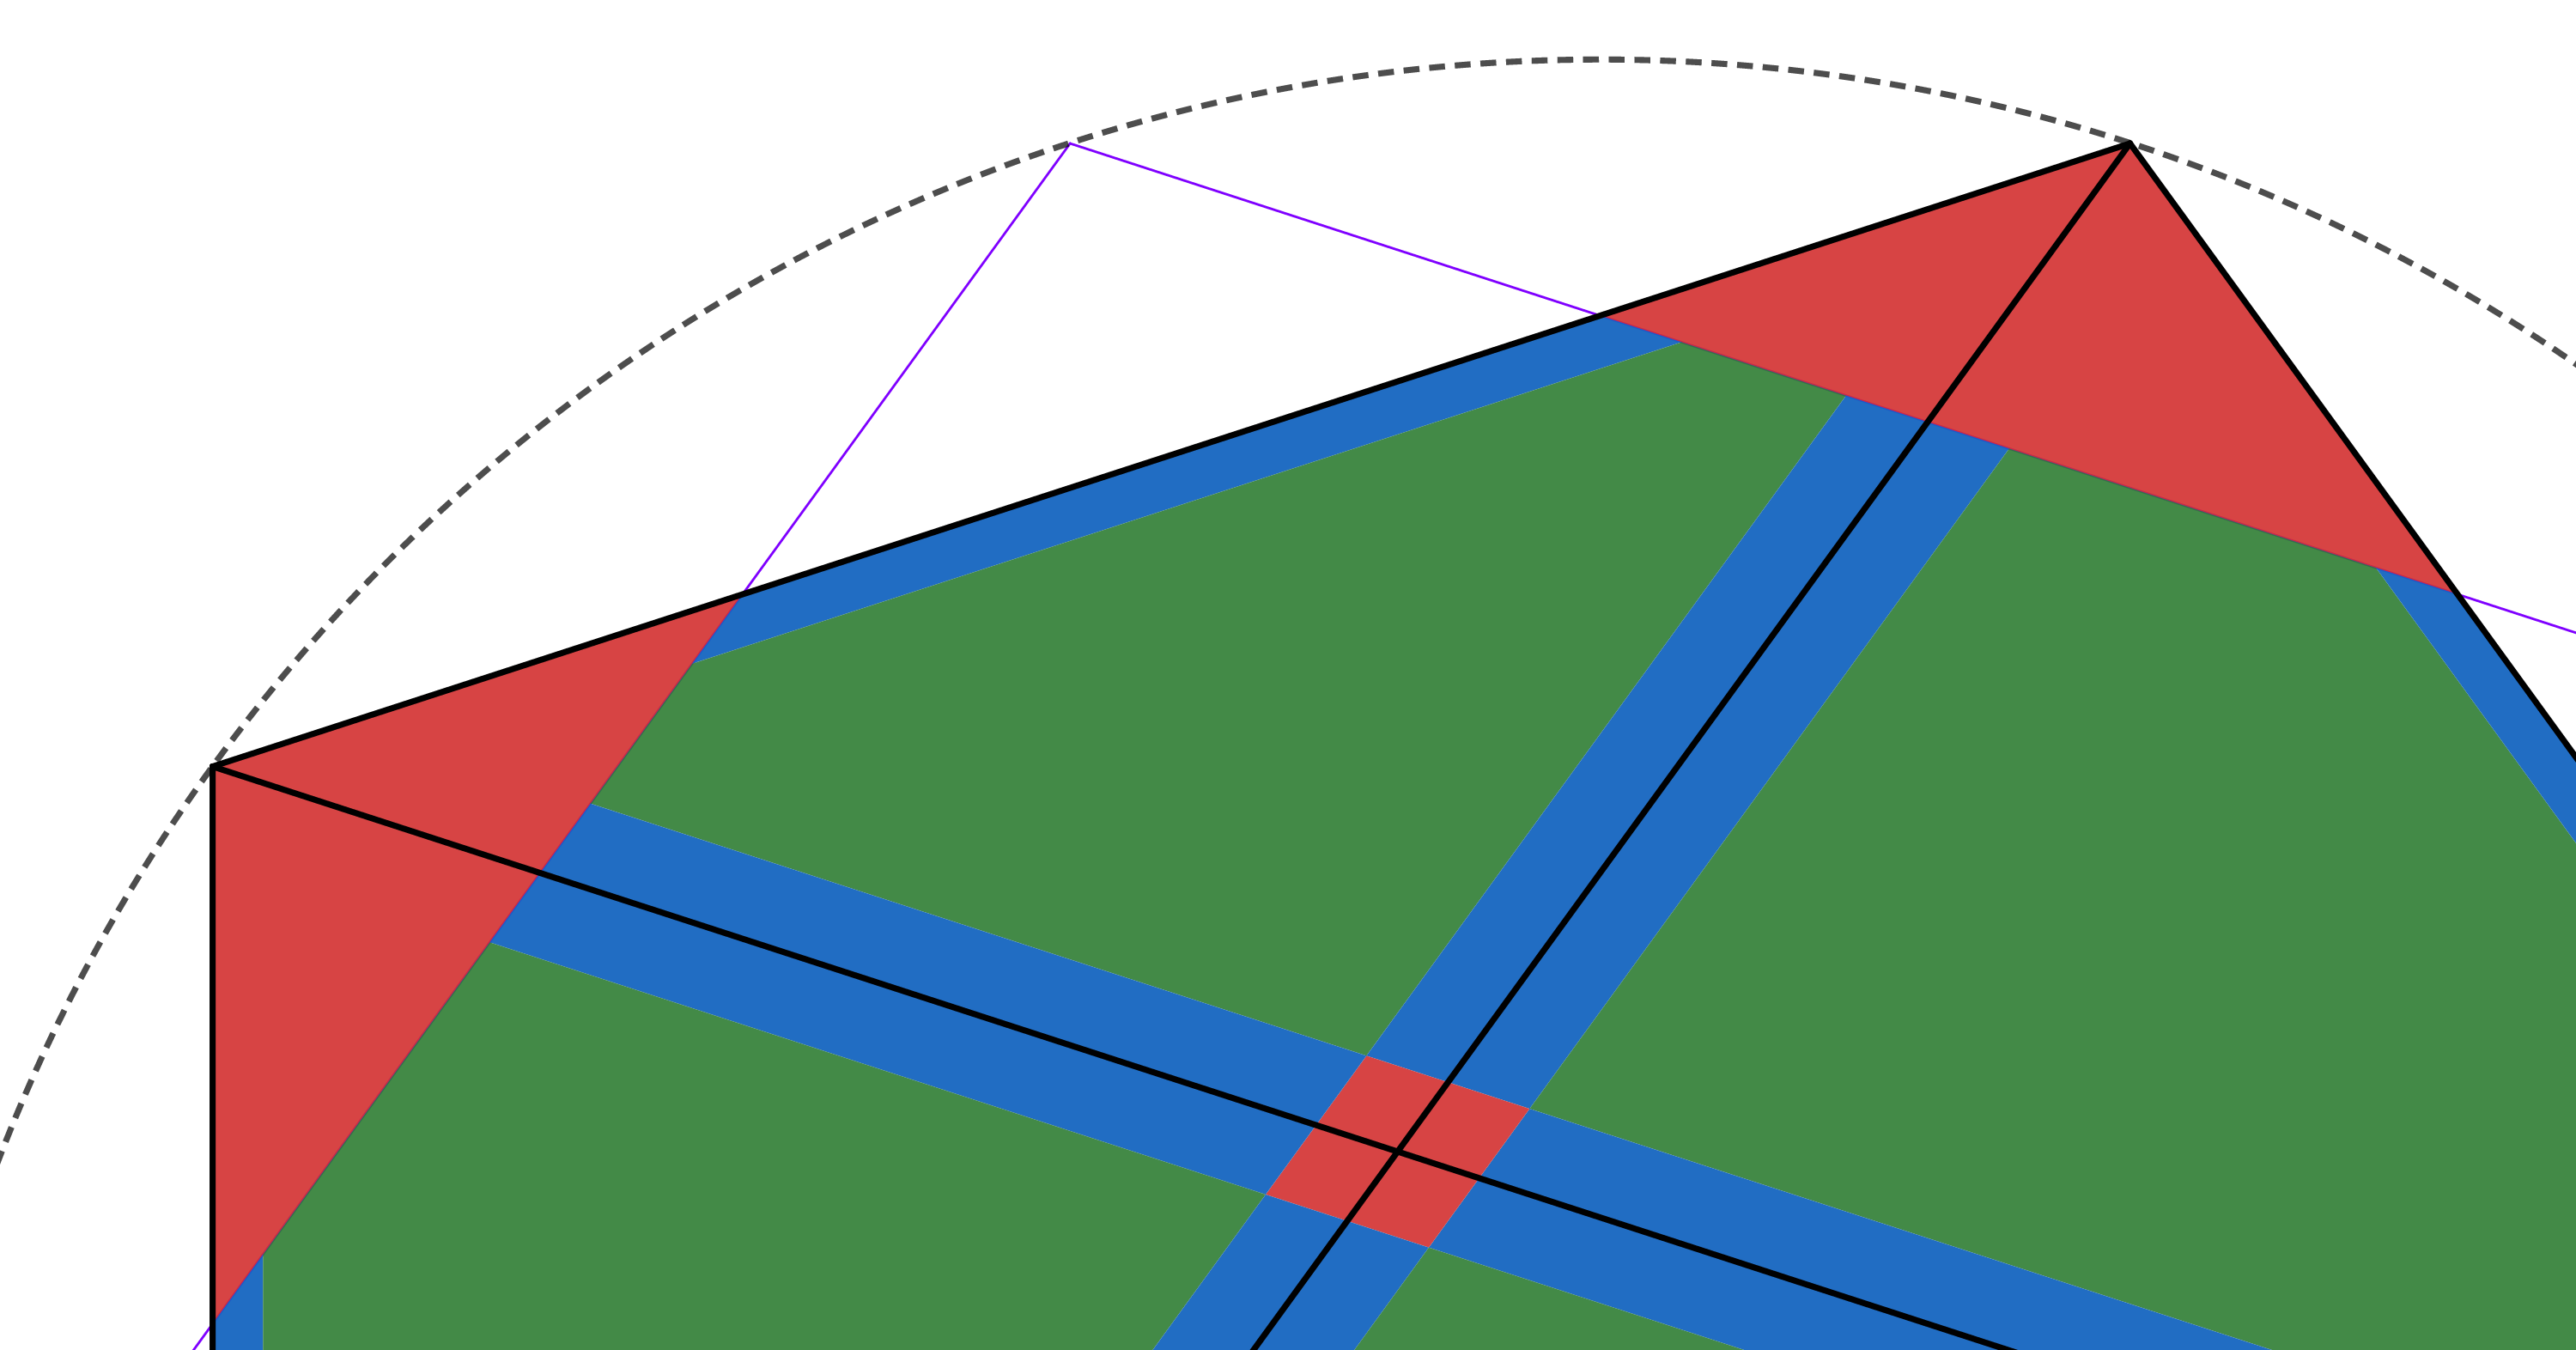
\includegraphics[width=0.9\textwidth]{figures/pl-segments-zoom.png}
	\caption{
		\textbf{A magnification of vertex and edge sleeve boundaries from Figure \ref{fig:pl-segments}.}
		A boundary combinatorial vertex sleeve intersects combinatorial face and edge sleeves at intervals, while an internal vertex sleeve intersects face sleeves at points and edge sleeves at intervals.
	}
	\label{fig:pl-segments-zoom}
\end{figure}

Moving to internal transversal surfaces, observe that the topology of a surface above a transversal $\gamma$ traveling along the secant $f(e)$ changes only when $\gamma$ encounters a vertex sleeve, so we need only examine the surfaces $f\inv(\gamma)$ when $\gamma$ lies on the boundary of a vertex sleeve.
Let $H$ be a vertex block, $f(H)$ the internal sleeve below $H$, and $e,e'$ the pair of edges of $N$ whose crossing induced the vertex sleeve.
Then $f(H)$ has boundary constructed from transversals over $e,e'$, two from each edge on opposite sides of $f(H)$, and we'll call these transversals $\gamma_i$, $i=1:4$.
Then $f\inv(\gamma_i)$ is a disjoint collection of triangulated surfaces in $M$ for each $i$, and we'll denote the surface incident with $H$ by
\[
	\Sigma_i = H\cap f\inv(\gamma_i).
\]
Then the boundary of $H$ is given by
\[
	\pd H = \bigcup_{i=1}^4 \Sigma_i.
\]
Now suppose $\Sigma_i$ has genus at least 1 for some $i$.
This means there is a pair of curves $J,K$ in $\Sigma_i$ that are essential in the surface formed by filling in the boundary components of $\Sigma_i$ with discs, the oriented intersection number of $J$ and $K$ is exactly 1, and $J\cup K$ is disjoint from the surfaces $\Sigma_j$ for $j\neq i$.
The vertex block $H$ is a triangulated (3,1)--handlebody, so one of $J,K$ is meridinal in $H$, say $J$.

The block $H$ is a (3,1)--handlebody because $H$ is a regular neighbourhood of the triangulated wedge of circles above $f(e_1)\cap f(e_2)$ in $M$, so all meridinal discs of $H$ are mapped bijectively to the vertex sleeve $f(H)$.
Specifically, meridians of $H$ are mapped bijectively to $\pd f(H) = \cup_i\gamma_i$, but $J$ is a meridian and $f(J)\subseteq \gamma_i$ for a single $\gamma_i$.
This is a contradiction, hence the genus of $\Sigma_i$ is 0 for each $i$, therefore $\Sigma_i$ is a (multiply) punctured 2--sphere for each $i$.

%
%Projecting $H$ through $f$ yields the vertex sleeve under $H$, and the boundary of this sleeve 
%
%
%The boundary $\pd H$ is a triangulated surface and $f(\pd H)$ projects over four edge sleeve boundaries, hence $\pd H = \bigcup_{i}f\inv(\gamma_i)$
%The block $H$ is the (3,1)--handlebody bounded by $\pd H$, and every meridinal disc of $H$ projects over the vertex sleeve that lies under $H$ in the plane, hence 
%Supposing 

%We subdivide $M$ iThe simplest subdivision method that is sufficient for our purposes and is more efficient than a barycentric subdivision is de
%For each 
%
%The Cartesian product of a pair of cell complexes is again a cell complex, so we form the base 4--dimensional cell-complex to which we attach handles as $M\times\Ilit$.
%Every cell of $M\times\Ilit$ is homeomorphic to a disk, so we form a 4--manifold triangulation $W$ as a subdivision of $M\times\Ilit$.
%This triangulation is obtained by inductively subdividing each cell of $M\times\Ilit$ that is not a simplex.




%Each 3--cell of $M$ maps through $f$ to a connected component of $f(N)\setminus f(N^1)$.
%Let $r$ be a connected component of $f(N)\setminus f(N^1)$.
%Then $f\inv(r)$ is a collection of 2-- and 3--cells in $M$ that form a  
%Their is a correspondence between the 3--cells of $M$ and the connected components of $f(N)\setminus f(N^1)$, and that correspondence 
%
%Decomposition of $\RR$ is done through $f(N_1)$.
%A point in $f(N_1)$ is the image of either a vertex, exactly one edge, or exactly two edges (i.e.\ is an edge crossing), so we refer to these as the \emph{vertices}, \emph{edges}, and \emph{crossings} of the decomposition.
%Because $f(N)\setminus f(N_1)$  is a disjoint collection of simply connected regions, we call the connected components of $f(N)\setminus f(N_1)$ the \emph{faces} of the decomposition.
%
%We construct our subdivision of $N$ using the decomposition component preimages.
%The preimage of a face component defines substructures analogous to face blocks, of edge components to edge blocks, and vertices and crossings to vertex blocks.
%Inside of an individual tetrahedron of $N$, edge and crossing preimages are well-defined, supplying a natural subdivision of $N$ into a cell complex.
%Then, the subdivision of a cell complex into a triangulation is well-defined.
%
%The algorithm presented in this section takes as input a closed, orientable 3--manifold triangulation $N$ and a projection $f:N\to\RR$ and produces as output a closed, orientable 3--dimensional cell complex $M$ that is a subdivision of $N$.
%Furthermore, the 3--cells of $M$ are partitioned into subsets that serve the same purpose as the face blocks of Chapter \ref{chapter:smooth}: attaching regions for 2--handles.
%This 3--cell partitioning also induces a partition on the 2--cells of $M$ into subsets that are either interior to face blocks, or subsets that serve the same purpose as the edge blocks of Chapter ~\ref{chapter:smooth}, i.e.\ buffers between face blocks.
%
%
%
%
%
